%% abtex2-modelo-trabalho-academico.tex, v-1.9.6 laurocesar
%% Copyright 2012-2016 by abnTeX2 group at http://www.abntex.net.br/ 
%%
%% This work may be distributed and/or modified under the
%% conditions of the LaTeX Project Public License, either version 1.3
%% of this license or (at your option) any later version.
%% The latest version of this license is in
%%   http://www.latex-project.org/lppl.txt
%% and version 1.3 or later is part of all distributions of LaTeX
%% version 2005/12/01 or later.
%%
%% This work has the L PPL maintenance status `maintained'.
%% 
%% The Current Maintainer of this work is the abnTeX2 team, led
%% by Lauro César Araujo. Further information are available on 
%% http://www.abntex.net.br/
%%
%% This work consists of the files abntex2-modelo-trabalho-academico.tex,
%% abntex2-modelo-include-comandos and abntex2-modelo-references.bib
% ------------------------------------------------------------------------
% ------------------------------------------------------------------------
% abnTeX2: Modelo de Trabalho Academico (tese de doutorado, dissertacao de
% mestrado e trabalhos monograficos em geral) em conformidade com 
% ABNT NBR 14724:2011: Informacao e documentacao - Trabalhos academicos -
% Apresentacao
% ------------------------------------------------------------------------
% ------------------------------------------------------------------------
% Personalização para o modelo Udesc 2024 9. ed. revisada e modificada
% Manual_13_05_2024_17175220258266_12510.pdf acesso em: 13/08/2024
% Autor: Felipe Joel Zimann (felipezimann@hotmail.com)
% Data: 02/12/2020 v1.0
% Data: 13/02/2021 v1.0.1 alterado tamanho numeração da página para 10pt
% Data: 13/08/2024 v1.0.2 alterado para citação (Autor, Ano) ao invés de (AUTOR, Ano) conforme ABNT NBR 10520:2023
% ------------------------------------------------------------------------
% ------------------------------------------------------------------------

\documentclass[
	12pt,					% tamanho da fonte
	openright,				% capítulos começam em pág ímpar (insere página vazia caso preciso)
	oneside,				% para impressão em recto e verso (twoside). Oposto a (oneside)
	a4paper,				% tamanho do papel. 
	chapter=TITLE,			% títulos de capítulos convertidos em letras maiúsculas
	section=TITLE,			% títulos de seções convertidos em letras maiúsculas
	sumario=abnt-6027-2012,
	english,				% idioma adicional para hifenização
	brazil,					% o último idioma é o principal do documento
	fleqn,					% equações alinhadas a esquerda (UDESC/CCT)+
	]{abntex2}

% ----------------------------------------------------------
% Pacotes básicos 
% ----------------------------------------------------------
\usepackage{amsmath}							% Pacote matemático
% \usepackage{amssymb}							% Pacote matemático
% \usepackage{amsfonts}							% Pacote matemático
%\usepackage{lmodern}							% Usa a fonte Latin Modern		
% \usepackage{mathptmx} 							% Usa a fonte Times New Roman	 (UDESC/CCT)
% \usepackage[T1]{fontenc}						% Selecao de codigos de fonte.
% \usepackage[utf8]{inputenc}						% Codificacao do documento (conversão automática dos acentos)
% \usepackage{lastpage}							% Usado pela Ficha catalográfica
\usepackage{indentfirst}						% Indenta o primeiro parágrafo de cada seção.
% \usepackage[dvipsnames,table]{xcolor}			% Controle das cores
% \usepackage{graphicx}							% Inclusão de gráficos
\usepackage{microtype} 							% para melhorias de justificação
% \usepackage{lipsum}								% para geração de dummy text
\usepackage[brazilian,hyperpageref]{backref}	% Paginas com as citações na bibl
\usepackage[alf,abnt-emphasize=bf,abnt-full-initials=yes]{abntex2cite}					% Citações padrão ABNT
%\usepackage[num]{abntex2cite}					% Citações padrão ABNT numérica
% \usepackage{adjustbox}							% Pacote de ajuste de boxes
% \usepackage{subcaption}							% Inclusão de Subfiguras e sublegendas		
% \usepackage{enumitem}							% Personalização de listas
\usepackage{siunitx}							% Grandezas e unidades
% \usepackage[section]{placeins}					% Manter as figuras delimitadas na respectiva seção com a opção [section]
\usepackage{multirow}							% Multi colunas nas tabelas
\usepackage{array,tabularx} 					% Pacotes de tabelas
\usepackage{booktabs}							% Pacote de tabela profissonal
% \usepackage{rotating}							% Rotacionar figuras e tabelas
% \usepackage{xfrac}								% Fazer frações n/d em linha
% \usepackage{bm}									% Negrito em modo matemático
% \usepackage{xstring}							% Manipulação de strings
\usepackage{pgfplots}							% Pacote de Gráficos
\usepackage{tikz}								% Pacote de Figuras
\usepackage[american, cuteinductors,smartlabels, fulldiode, siunitx, americanvoltages, oldvoltagedirection, smartlabels]{circuitikz}						% Pacote de circuitos elétricos
\usepackage{chemformula}						% Pacote para fórmulas químicas
\usepackage{chngcntr}							% Pacte usado para deixar numeração de equações sequencial (UDESC/CCT)
\counterwithout{equation}{chapter}
% fonte: https://latex.org/forum/viewtopic.php?t=15392

% Comando para deixar numeração das equações contínua (1), (2), (3)... ao invés de organizar por capítulos (1.1)(1.2)... (2.1)(2.2)
%\renewcommand{\theequation}{\arabic{equation}}

%\numberwithin{equation}{section}


% Cabecalho cabeçalho somente com numeração de página 10pt
\makepagestyle{PagNumReduzida}
\makeevenhead{PagNumReduzida}{\ABNTEXfontereduzida\thepage}{}{}
\makeoddhead{PagNumReduzida}{}{}{\ABNTEXfontereduzida\thepage}
%fonte: https://github.com/abntex/abntex2/wiki/HowToCustomizarCabecalhoRodape
%fonte: Manual memoir seção 7.3 pg. 111 pdf http://linorg.usp.br/CTAN/macros/latex/contrib/memoir/memman.pdf 

% Personalização das opções das listas
\setlist[itemize]{leftmargin=\parindent}

% Citação online --- MODIFICAR ---
\newcommand{\citeshort}[1]{\citeauthoronline{#1}~(\citeyear{#1})}

\newcommand{\me}[1]{Elaborado pelo autor (#1).}

% Configuração do pgfplots
\pgfplotsset{compat=newest} %compat=1.14
\pgfplotsset{plot coordinates/math parser=false} 
\newlength\figureheight 
\newlength\figurewidth 

% % Libraries do TiKz
% \usetikzlibrary{quotes,angles,arrows}
% \usetikzlibrary{through,calc,math}
% \usetikzlibrary{graphs,backgrounds,fit}
% \usetikzlibrary{shapes,positioning,patterns,shadows}
% \usetikzlibrary{decorations.pathreplacing}
% \usetikzlibrary{shapes.geometric}
% \usetikzlibrary{arrows.meta}
% \usetikzlibrary{external}

% %\tikzexternalize[]
% %\tikzexternalenable
% %\tikzexternalize
% %\tikzexternaldisable
% %\tikzset{external/force remake}
% %\tikzexternalize[shell escape=-enable-write18]

% % Configurações do CircuiTiKz
% \ctikzset{bipoles/thickness=1}
% %\ctikzset{bipoles/length=1.2cm}
% \ctikzset{monopoles/ground/width/.initial=.2}
% \ctikzset{bipoles/resistor/height=0.25}
% \ctikzset{bipoles/resistor/width=0.6}
% \ctikzset{bipoles/capacitor/height=0.5}
% \ctikzset{bipoles/capacitor/width=0.15}
% \ctikzset{bipoles/generic/height=0.25}
% \ctikzset{bipoles/generic/width=0.6}
% %\ctikzset{bipoles/capacitor polar/length=0.5}
% %\ctikzset{bipoles/diode/height=.375}
% %\ctikzset{bipoles/diode/width=.3}
% %\ctikzset{tripoles/thyristor/height=.8}
% %\ctikzset{tripoles/thyristor/width=1}
% \ctikzset{bipoles/vsourcesin/height=.5}
% \ctikzset{bipoles/vsourcesin/width=.5}
% \ctikzset{bipoles/cvsourceam/height=.6}
% \ctikzset{bipoles/cvsourceam/width=.6}
% %\ctikzset{tripoles/european controlled voltage source/width=.4}

% \tikzstyle{every node}=[font=\footnotesize]
% \tikzstyle{every path}=[line width=0.25pt,line cap=round,line join=round]
%\tikzstyle{every path}=[line cap=round,line join=round]


% Definição de cores MATLAB
\definecolor{matlab_blue}{rgb}	{         0,    0.4470,    0.7410}
\definecolor{matlab_orange}{rgb}{    0.8500,    0.3250,    0.0980}
\definecolor{matlab_yellow}{rgb}{    0.9290,    0.6940,    0.1250}
\definecolor{matlab_violet}{rgb}{    0.4940,    0.1840,    0.5560}
\definecolor{matlab_green}{rgb}	{	 0.4660,    0.6740,    0.1880}
\definecolor{matlab_lblue}{rgb}	{    0.3010,    0.7450,    0.9330}
\definecolor{matlab_red}{rgb}	{    0.6350,    0.0780,    0.1840}

% Personalização das legendas
\usepackage[format = plain, %hang
			justification = centering,
			labelsep = endash,
			singlelinecheck = false,
			skip = 6pt,
			listformat = simple]{caption}	

% Personalização das unidades
\sisetup{output-decimal-marker = {,}}
\sisetup{exponent-product = \cdot}
\sisetup{tight-spacing=true}
\sisetup{group-digits = false}

% Personalizações de tipo de colunas de tabelas
\newcolumntype{L}[1]{>{\raggedright\let\newline\\\arraybackslash\hspace{0pt}}m{#1}}
\newcolumntype{C}[1]{>{\centering\let\newline\\\arraybackslash\hspace{0pt}}m{#1}}
\newcolumntype{R}[1]{>{\raggedleft\let\newline\\\arraybackslash\hspace{0pt}}m{#1}}

% Personalizações de cores da UDESC
\definecolor{CapaAmareloUDESC}{RGB}{243,186,83}		% Especializacao
\definecolor{CapaVerdeUDESC}{RGB}{0,112,52}			% Mestrado
\definecolor{CapaVermelhoUDESC}{RGB}{171,35,21}		% Doutorado
\definecolor{CapaAzulUDESC}{RGB}{38,54,118} 		% Pós-Doutorado

% CONFIGURAÇÕES DE PACOTES
% Configurações do pacote backref
% Usado sem a opção hyperpageref de backref
\renewcommand{\backrefpagesname}{Citado na(s) página(s):~}
% Texto padrão antes do número das páginas
\renewcommand{\backref}{}
% Define os textos da citação
\renewcommand*{\backrefalt}[4]{
	\ifcase #1 %
	Nenhuma citação no texto.%
	\or
	Citado na página #2.%
	\else
	Citado #1 vezes nas páginas #2.%
	\fi}%

% alterando o aspecto da cor azul
%\definecolor{blue}{RGB}{41,5,195}

% informações do PDF
\makeatletter
\hypersetup{
	%pagebackref=true,
	pdftitle={\@title}, 
	pdfauthor={\@author},
	pdfsubject={\imprimirpreambulo},
	pdfcreator={LaTeX with abnTeX2},
	pdfkeywords={abnt}{latex}{abntex}{abntex2}{trabalho academico}, 
	colorlinks=true,       		% false: boxed links; true: colored links
	linkcolor=black,          	% color of internal links
	citecolor=black,        	% color of links to bibliography
	filecolor=black,      		% color of file links
	urlcolor=black,
	bookmarksdepth=4
}
\makeatother


\makeatletter
\newcommand{\includetikz}[1]{%
	\tikzsetnextfilename{#1}%
	\input{#1.tex}%
}
\makeatother


% ---
% Possibilita criação de Quadros e Lista de quadros.
% Ver https://github.com/abntex/abntex2/issues/176
%
\newcommand{\quadroname}{Quadro}
\newcommand{\listofquadrosname}{Lista de quadros}

\newfloat[chapter]{quadro}{loq}{\quadroname}
\newlistof{listofquadros}{loq}{\listofquadrosname}
\newlistentry{quadro}{loq}{0}

% configurações para atender às regras da ABNT
\setfloatadjustment{quadro}{\centering}
\counterwithout{quadro}{chapter}
\renewcommand{\cftquadroname}{\quadroname\space} 
\renewcommand*{\cftquadroaftersnum}{\hfill--\hfill}

\setfloatlocations{quadro}{hbtp} % Ver https://github.com/abntex/abntex2/issues/176
% ---


% Espaçamento depois do título
\setlength{\afterchapskip}{0.7\baselineskip}
% O tamanho do parágrafo é dado por:
\setlength{\parindent}{1.25cm}
% Controle do espaçamento entre um parágrafo e outro:
\setlength{\parskip}{0.0cm}  % tente também \onelineskip
%\SingleSpacing % Espaçamento simples 
\OnehalfSpacing % Espaçamento 1,5 (UDESC/CCT)
%\DoubleSpacing	% Espaçamento duplo

% ---
% Margens - NBR 14724/2011 - 5.1 Formato
% ---
\setlrmarginsandblock{3cm}{2cm}{*}
\setulmarginsandblock{3cm}{2cm}{*}
\checkandfixthelayout[fixed]
% ---


% To use externalize consider
%https://tex.stackexchange.com/questions/182783/tikzexternalize-not-compatible-with-miktex-2-9-abntex2-package
%Lauro Cesar digged into the problem until he came with a solution for me to test. And it Works!
%
%According to this link:
%
%The package calc changed the commands \setcounter and friends to be fragile. So you have to make them robust. The example below uses etoolbox with \robustify:
%
\usepackage{etoolbox}
\robustify\setcounter
\robustify\addtocounter
\robustify\setlength
\robustify\addtolength


%% How to silence memoir class warning against the use of caption package?
%% https://tex.stackexchange.com/questions/391993/how-to-silence-memoir-class-warning-against-the-use-of-caption-package
%\usepackage{silence}
%\WarningFilter*{memoir}{You are using the caption package with the memoir class}
%\WarningFilter*{Class memoir Warning}{You are using the caption package with the memoir class}

% --------------------------------------------------------
% INICIO DAS CUSTOMIZACOES PARA A UDESC
% --------------------------------------------------------

% --------------------------------------------------------
% Fontes padroes de part, chapter, section, subsection e subsubsection
% --------------------------------------------------------
% --- Chapter ---
\renewcommand{\ABNTEXchapterfont}{\fontseries{b}} %\bfseries
\renewcommand{\ABNTEXchapterfontsize}{\normalsize}
% --- Part ---
\renewcommand{\ABNTEXpartfont}{\ABNTEXchapterfont}
\renewcommand{\ABNTEXpartfontsize}{\LARGE}
% --- Section ---
\renewcommand{\ABNTEXsectionfont}{\normalfont}
\renewcommand{\ABNTEXsectionfontsize}{\normalsize}
% --- SubSection ---
\renewcommand{\ABNTEXsubsectionfont}{\fontseries{b}} %\bfseries
\renewcommand{\ABNTEXsubsectionfontsize}{\normalsize}
% --- SubSubSection ---
\renewcommand{\ABNTEXsubsubsectionfont}{\itshape}
\renewcommand{\ABNTEXsubsubsectionfontsize}{\normalsize}

\renewcommand{\ABNTEXsubsubsubsectionfont}{\normalfont}
\renewcommand{\ABNTEXsubsubsubsectionfontsize}{\normalsize}
% ---

% --------------------------------------------------------
% Fontes das entradas do sumario
% --------------------------------------------------------

\renewcommand{\cftpartfont}{\ABNTEXpartfont\selectfont}
\renewcommand{\cftpartpagefont}{\normalsize\selectfont}

\renewcommand{\cftchapterfont}{\ABNTEXchapterfont\selectfont}
\renewcommand{\cftchapterpagefont}{\normalsize\selectfont}

\renewcommand{\cftsectionfont}{\ABNTEXsectionfont\selectfont}
\renewcommand{\cftsectionpagefont}{\normalsize\selectfont}

\renewcommand{\cftsubsectionfont}{\ABNTEXsubsectionfont\selectfont}
\renewcommand{\cftsubsectionpagefont}{\normalsize\selectfont}

\renewcommand{\cftsubsubsectionfont}{\normalfont\itshape\selectfont}
\renewcommand{\cftsubsubsectionpagefont}{\normalsize\selectfont}

\renewcommand{\cftparagraphfont}{\normalfont\selectfont}
\renewcommand{\cftparagraphpagefont}{\normalsize\selectfont}

% --------------------------------------------------------
% Usando os pacotes hyperref, uppercase... 
% Para deixar a section do toc uppercase precisa de:
% --------------------------------------------------------
\usepackage{textcase}

\makeatletter

\let\oldcontentsline\contentsline
\def\contentsline#1#2{%
	\expandafter\ifx\csname l@#1\endcsname\l@section
	\expandafter\@firstoftwo
	\else
	\expandafter\@secondoftwo
	\fi
	{%
		\oldcontentsline{#1}{\MakeTextUppercase{#2}}%
	}{%
		\oldcontentsline{#1}{#2}%
	}%
}
\makeatother

% --------------------------------------------------------
% Renomenando as entradas de APÊNDICES E ANEXOS
% --------------------------------------------------------

\renewcommand{\apendicesname}{AP\^ENDICES}
\renewcommand{\anexosname}{ANEXOS}


% Manipulação de Strings
%\RequirePackage{xstring}

% Comando para inverter sobrenome e nome
\newcommand{\invertname}[1]{%
	\StrBehind{#1}{{}}, \StrBefore{#1}{{}}%
}%


% --------------------------------------------------------
% Alterando os estilos de Caption e Fonte
% --------------------------------------------------------
\makeatletter
% Define o comando \fonte que respeita as configurações de caption do memoir ou do caption
\renewcommand{\fonte}[2][\fontename]{%
	\M@gettitle{#2}%
	\memlegendinfo{#2}%
	\par
	\begingroup
	\@parboxrestore
	\if@minipage
	\@setminipage
	\fi
	\ABNTEXfontereduzida
	\configureseparator
	\captiondelim{\ABNTEXcaptionfontedelim}
	\@makecaption{#1}{\ignorespaces #2}\par
	\endgroup}


\captionstyle[\raggedright]{\raggedright}

\makeatother

\setlength{\cftbeforechapterskip}{0pt plus 0pt}
\renewcommand*{\insertchapterspace}{}

\newlength{\mylen}	% New length to use with spacing
\setlength{\mylen}{1pt}

\setlength{\cftbeforechapterskip}{\mylen}
\setlength{\cftbeforesectionskip}{\mylen}
\setlength{\cftbeforesubsectionskip}{\mylen}
\setlength{\cftbeforesubsubsectionskip}{\mylen}
\setlength{\cftbeforesubsubsubsectionskip}{\mylen}


% ---
% Ajuste das listas de abreviaturas e siglas ; e símbolos [Personalizada para UDESC com espaçamento 1,5]
% ---

% ---
% Redefinição da Lista de abreviaturas e siglas [Personalizada para UDESC com espaçamento 1,5]
\renewenvironment{siglas}{%
	\pretextualchapter{\listadesiglasname}
	\begin{symbols} 
		\setlength{\itemsep}{0pt}	% Ajuste para Espaçamento 1,5 (UDESC/CCT)
	}{% 
	\end{symbols}
	\cleardoublepage
}
% ---

% ---
% Redefinição da Lista de símbolos [Personalizada para UDESC com espaçamento 1,5]
\renewenvironment{simbolos}{%
	\pretextualchapter{\listadesimbolosname}
	\begin{symbols}
		\setlength{\itemsep}{0pt}	% Ajuste para Espaçamento 1,5 (UDESC/CCT)
	}{%
	\end{symbols}
	\cleardoublepage
}
% ---


% ---
% Remocao dos simbolos de < > das urls, ver manual pacote url pg 6 item 6
% https://github.com/abntex/biblatex-abnt/issues/16
\def\UrlLeft{}
\def\UrlRight{}
% ---

% ---
% FIM DAS CUSTOMIZACOES PARA A  Universidade do Estado de Santa Catarina - UDESC/CCT
% ---





	% Incliu pacotes básicos 

% -----------------------------------------------------------------
% Você pode adicionar seus pacotes a partir desta linha;
% -----------------------------------------------------------------

%\usepackage[showframe,pass]{geometry}
%\usepackage[11,12]{pagesel}

% -----------------------------------------------------------------
% Informações de dados para CAPA e FOLHA DE ROSTO
% -----------------------------------------------------------------
\titulo{Projeto de um sistema de refrigeração}%

\autor{André Luiz {}Floriano \\ Antonio Vinícius Souza Menezes}%
\orientador{Sherlock Holmes {}da Silva}%
\coorientador{Arnold Alois {}Schwarzenegger}%

% ATENÇÃO: O símbolo {} indica o sobrenome para a ficha catalográfica.
% Exemplo: Sherlock Holmes {}da Silva para sobrenomes compostos;
% Exemplo: Arnold Alois {}Schwarzenegger para sobrenome simples.

\instituicao{Universidade do Estado de Santa Catarina, Centro de Ciências Tecnológicas, Programa de Graduação em Engenharia Mecânica}%

%\tipotrabalho{Tese (Doutorado)}
\tipotrabalho{Dissertação (Mestrado)}

%\preambulo{Tese apresentada ao Programa de Pós--Graduação em Engenharia Elétrica do Centro de Ciências Tecnológicas da Universidade do Estado de Santa Catarina, como requisito parcial para a obtenção do grau de Doutor em Engenharia Elétrica.}

\preambulo{Dissertação apresentada ao Programa de Pós--Graduação em Engenharia Elétrica do Centro de Ciências Tecnológicas da Universidade do Estado de Santa Catarina, como requisito parcial para a obtenção do grau de Mestre em Engenharia Elétrica.}

\local{Joinville}%

\data{\the\year}%
% ---

% compila o indice
\makeindex

% -----------------------------------------------------------------
% Início do documento
% -----------------------------------------------------------------
\begin{document}

\selectlanguage{brazil}
\frenchspacing  % Retira espaço extra obsoleto entre as frases.

% -----------------------------------------------------------------
% ELEMENTOS PRÉ-TEXTUAIS
% -----------------------------------------------------------------
\pretextual

% Você pode comentar os elementos que não deseja em seu trabalho;

% A capa pode ser escolhida dentro do arquivo Capa.tex (TCC, Master, Doc, ...)
% ---
% Capa
% ---


% --------------------------------------------------------
% Capa Padrão
% --------------------------------------------------------
\renewcommand{\imprimircapa}{%
	\begin{capa}%
		\center

		{\fontseries{b}\selectfont\MakeTextUppercase{UNIVERSIDADE DO ESTADO DE SANTA CATARINA -- UDESC}}
		
		{\fontseries{b}\selectfont\MakeTextUppercase{CCT}}
		
		{\fontseries{b}\selectfont\MakeTextUppercase{PROGRAMA DE GRADUAÇÃO EM ENGENHARIA MECÂNICA}}
		
		\vfill
		
		{\fontseries{b}\selectfont\MakeTextUppercase{\normalsize\imprimirautor}}
		
		\vfill
		\begin{center}
			{\fontseries{b}\selectfont\MakeTextUppercase{\imprimirtitulo}}
		\end{center}
		\vfill
		
		\vfill
		
		{\fontseries{b}\selectfont\MakeTextUppercase{\imprimirlocal}}
		\par
		{\fontseries{b}\selectfont \imprimirdata}
		\vspace*{1cm}
	\end{capa}
}



\imprimircapa				% Capa padrão

					% Elemento Obrigatório
% % ---
% Folha de rosto
% ---








% --------------------------------------------------------
% folha de rosto 
% --------------------------------------------------------

\makeatletter

\renewcommand{\folhaderostocontent}{
	\begin{center}
		
		{\fontseries{b}\selectfont\MakeTextUppercase{\imprimirautor}}
		
		\vfill
		
		\begin{center}
			{\fontseries{b}\selectfont\MakeTextUppercase{\imprimirtitulo}}
		\end{center}
	
		\vspace*{1.5cm}

		\abntex@ifnotempty{\imprimirpreambulo}{%
			\hspace{.45\textwidth}
			{\begin{minipage}{.5\textwidth}
					\SingleSpacing
					\imprimirpreambulo\par
					\vspace*{4pt}
					{\imprimirorientadorRotulo~\imprimirorientador\par}
					\abntex@ifnotempty{\imprimircoorientador}{%
						{\imprimircoorientadorRotulo~\imprimircoorientador}%
					}%
			\end{minipage}}%
		}%
	
		
		\vfill
		
	{\fontseries{b}\selectfont\MakeTextUppercase{\imprimirlocal}}
	\par
	{\fontseries{b}\selectfont \imprimirdata}
	\vspace*{1cm}
	\end{center}
}


% (o * indica que haverá a ficha bibliográfica)
% ---
\imprimirfolhaderosto*
% ---


			% Elemento Obrigatório
% Caso não utilize a Ficha Catalográfica entre na folha de rosto e retire o * de dentro do arquivo FolhadeRosto
% 
% ---
% Inserir a ficha bibliografica
% ---

% Isto é um exemplo de Ficha Catalográfica, ou ``Dados internacionais de
% catalogação-na-publicação''. Você pode utilizar este modelo como referência. 
% Porém, provavelmente a biblioteca da sua universidade lhe fornecerá um PDF
% com a ficha catalográfica definitiva após a defesa do trabalho. Quando estiver
% com o documento, salve-o como PDF no diretório do seu projeto e substitua todo
% o conteúdo de implementação deste arquivo pelo comando abaixo:



% \begin{fichacatalografica}
%     \includepdf{fig_ficha_catalografica.pdf}
% \end{fichacatalografica}


%	\setlength{\parindent}{0cm}
%	\setlength{\parskip}{0pt}
\begin{fichacatalografica}
	%\sffamily
	%\rmfamily
	%\ttfamily 
	\hbadness=10000
	\vspace*{\fill}					% Posição vertical
	\begin{center}					% Minipage Centralizado
	Para gerar a ficha catalográfica de teses e \\ 
	dissertações acessar o link:  \\
	https://www.udesc.br/bu/manuais/ficha
	
	\vspace*{8pt}
	
%	\begin{minipage}[c]{8cm}
%	\centering \sffamily
%	 Ficha catalográfica elaborada pelo(a) autor(a), com auxílio do programa de geração automática da Biblioteca Setorial do CCT/UDESC
%	\end{minipage}
	\fbox{\begin{minipage}[c]{13.5cm}		% Largura
	\flushright
	{\begin{minipage}[c]{10.5cm}		% Largura
	\vspace{1.25cm}
	%\footnotesize
	\setlength{\parindent}{1.5em}
	\noindent \invertname{\imprimirautor} \par
	\imprimirtitulo{ }/{ }\imprimirautor. -- \imprimirlocal, \imprimirdata .\par
	\pageref{LastPage} p. : il. \par
	\vspace{1.5em}
	\imprimirorientadorRotulo~\imprimirorientador.\par
	\imprimircoorientadorRotulo~\imprimircoorientador.\par
	\imprimirtipotrabalho~--~\imprimirinstituicao, \imprimirlocal, \imprimirdata.\par
	\vspace{1.5em}
		1. Palavra-chave.
		2. Palavra-chave.
		3. Palavra-chave.
 		4. Palavra-chave.
		5. Palavra-chave.
		I. \invertname{\imprimirorientador}.
		II. \invertname{\imprimircoorientador}.
		III. \imprimirinstituicao.
		IV. Título. %
	\vspace{1.25cm}	%		
	\end{minipage}%
	}% 
	\hspace{10mm}
	\end{minipage}}%
	
	\vspace*{0.5cm}
	
	\end{center}
\end{fichacatalografica}


%\begin{fichacatalografica}
%	\sffamily
%	\vspace*{\fill}					% Posição vertical
%	\begin{center}					% Minipage Centralizado
%	\fbox{\begin{minipage}[c][8cm]{13.5cm}		% Largura
%	\small
%	\imprimirautor
%	%Sobrenome, Nome do autor
%	
%	\hspace{0.5cm} \imprimirtitulo  / \imprimirautor. --
%	\imprimirlocal, \imprimirdata-
%	
%	\hspace{0.5cm} \pageref{LastPage} p. : il. (algumas color.) ; 30 cm.\\
%	
%	\hspace{0.5cm} \imprimirorientadorRotulo~\imprimirorientador\\
%	
%	\hspace{0.5cm}
%	\parbox[t]{\textwidth}{\imprimirtipotrabalho~--~\imprimirinstituicao,
%	\imprimirdata.}\\
%	
%	\hspace{0.5cm}
%		1. Palavra-chave1.
%		2. Palavra-chave2.
%		3. Palavra-chave3.
% 		4. Palavra-chave4.
%		5. Palavra-chave5.
%		I. Orientador.
%		II. Universidade xxx.
%		III. Faculdade de xxx.
%		IV. Título 			
%	\end{minipage}}
%	\end{center}
%\end{fichacatalografica}
% ---

	% Elemento Obrigatório (Verso da Folha)
% 
% ---
% Inserir errata
% ---
\begin{errata}
Elemento opcional. 

Exemplo:

\vspace{\onelineskip}

Sobrenome, Prenome do Autor. Título de obra: subtítulo (se houver). Ano de depósito. Tipo do trabalho (grau e curso) - Vinculação acadêmica, local de apresentação/defesa, data.

\begin{table}[htb]
\center
\begin{tabular}{|p{2.4cm}|p{2cm}|p{3cm}|p{3cm}|}
  \hline
   \textbf{Folha} & \textbf{Linha}  & \textbf{Onde se lê}  & \textbf{Leia-se}  \\
    \hline
    1 & 10 & auto-conclavo & autoconclavo\\
   \hline
\end{tabular}
\end{table}

\end{errata}
% ---				% Elemento Opcional
% 
% ---
% Inserir folha de aprovação
% ---

% Isto é um exemplo de Folha de aprovação, elemento obrigatório da NBR
% 14724/2011 (seção 4.2.1.3). Você pode utilizar este modelo até a aprovação
% do trabalho. Após isso, substitua todo o conteúdo deste arquivo por uma
% imagem da página assinada pela banca com o comando abaixo:
%
% \includepdf{folhadeaprovacao_final.pdf}
%
\begin{folhadeaprovacao}



	\begin{center}
		{\fontseries{b}\selectfont\MakeTextUppercase{\normalsize\imprimirautor}}
	\end{center}
    \vfill
    
	\vfill
	\begin{center}
		{\fontseries{b}\selectfont\MakeTextUppercase{\imprimirtitulo}}
	\end{center}
	\vfill

    
\abntex@ifnotempty{\imprimirpreambulo}{%
	\hspace{.45\textwidth}
	{\begin{minipage}{.5\textwidth}
			\SingleSpacing
			\imprimirpreambulo\par
			\vspace*{4pt}
			{\imprimirorientadorRotulo~\imprimirorientador\par}
			\abntex@ifnotempty{\imprimircoorientador}{%
				{\imprimircoorientadorRotulo~\imprimircoorientador}%
			}%
	\end{minipage}}%
}%


\vfill
        
	 \begin{center}
	 	
    	{\fontseries{b}\selectfont BANCA EXAMINADORA: }
    	\vspace*{1.75cm}
    
		Nome do Orientador e Titulação \par
		Nome da Instituição
	 \end{center}
	
    {Membros:} 
    
	\begin{center}
		\vspace*{1.25cm}
		Nome do Orientador e Titulação \par
		Nome da Instituição
		
		\vspace*{1.25cm}
		Nome do Orientador e Titulação \par
		Nome da Instituição
		
		\vspace*{1.25cm}
		Nome do Orientador e Titulação \par
		Nome da Instituição

	
	\end{center}
    
    \vspace*{\fill}  
    \begin{center}
    {\imprimirlocal, 01 de maio de \imprimirdata}
	\end{center}
    \vspace*{0.25cm}  
\end{folhadeaprovacao}
% ---




%\textbf{	{Orientador: \vspace{-16pt} }
%	\assinatura{\textbf{Prof. \imprimirorientador , Dr.} \\ Univ. XXX} 
%	{Coorientador: \vspace{-16pt}}   
%	\assinatura{\textbf{Prof. \imprimircoorientador , Dr.} \\ Univ. XXX}
%	
%	{Membros: \vspace{-16pt} } 
%	
%	% --- Exemplo de assinaturas em sequência ---       
%	\setlength{\ABNTEXsignwidth}{8.5cm}
%	
%	\assinatura{\textbf{Prof. Professor, Dr.} \\ Univ. XXX}
%	\assinatura{\textbf{Prof. Professor, Dr.} \\ Univ. XXX}
%	\assinatura{\textbf{Prof. Professor, Dr.} \\ Univ. XXX}
%	
%	% --- Exemplo de assinaturas lado a lado ---
%	\setlength{\ABNTEXsignwidth}{7.5cm}
	%
	%    \noindent\hfill\assinatura*{\textbf{Prof. Professor, Dr.} \\ Univ. XXX}%
	%    \hfill%
	%    \assinatura*{\textbf{Prof. Professor, Dr.} \\ Univ. XXX}%
	%    \hfill
	%    
	%    \noindent\hfill\assinatura*{\textbf{Prof. Professor, Dr.} \\ Univ. XXX}%
	%    \hfill%
	%    \assinatura*{\textbf{Prof. Professor, Dr.} \\ Univ. XXX}%
	%    \hfill}		% Elemento Obrigatório
% % ---
% Dedicatória
% ---
\begin{dedicatoria}
   \vspace*{\fill}
%   \begin{flushright}
%   \noindent
%	Este trabalho é dedicado às crianças adultas que,\\
%	quando pequenas, sonharam em se tornar cientistas. 
%   \end{flushright}

{%
	\noindent\hspace{.5\textwidth}
	{\begin{minipage}{.5\textwidth}
			\begin{flushleft}
				Aos estudantes da Universidade do Estado de Santa Catarina, pela inspiração de sempre!
			\end{flushleft}
	\end{minipage}}%
\vspace*{3cm}
}%

\end{dedicatoria}
% ---
			% Elemento Opcional
% % ---
% Agradecimentos
% ---
\begin{agradecimentos}
Agradeço ao meu orientador por aceitar conduzir o meu trabalho de pesquisa.
A todos os meus professores do curso de da Universidade do Estado de Santa Catarina – Udesc pela excelência da qualidade técnica de cada um.

Aos meus pais que sempre estiveram ao meu lado me apoiando ao longo de toda a minha trajetória. Sou grato à minha família pelo apoio que sempre me deram durante toda a minha vida.

Como disse Snoop Dog: ``Eu quero me agradecer por acreditar em mim mesmo, quero me agradecer por todo esse trabalho duro. Quero me agradecer por não tirar folgas. Quero me agradecer por nunca desistir. Quero me agradecer por ser generoso e sempre dar mais do que recebo. Quero me agradecer por tentar sempre fazer mais o certo do que o errado. Quero me agradecer por ser eu mesmo o tempo inteiro''.

Deixo um agradecimento especial ao meu orientador pelo incentivo e pela dedicação do seu escasso tempo ao meu projeto de pesquisa.


\end{agradecimentos}
% ---		% Elemento Opcional
% % ---
% Epígrafe
% ---
\begin{epigrafe}
    \vspace*{\fill}
%	\begin{flushright}
%		\textit{``Eu não falhei, encontrei 10 mil soluções que não davam certo.'' (EDISON, [19--])}
%	\end{flushright}
{%
	\noindent\hspace{.5\textwidth}
	{\begin{minipage}{.5\textwidth}
		\begin{flushright}
			``Eu não falhei, encontrei 10 mil soluções que não davam certo.'' (Edison, [19--])
		\end{flushright}
	\end{minipage}}%
	\vspace*{3cm}
}%
\end{epigrafe}
% ---				% Elemento Opcional
% % ---
% RESUMOS
% ---

% resumo em português
\setlength{\absparsep}{18pt} % ajusta o espaçamento dos parágrafos do resumo
\begin{resumo}
Elemento obrigatório que contém a apresentação concisa dos pontos relevantes do trabalho, fornecendo uma visão rápida e clara do conteúdo e das conclusões do mesmo. A apresentação e a redação do resumo devem seguir os requisitos estipulados pela NBR 6028 (ABNT, 2003). Deve descrever de forma clara e sintética a natureza do trabalho, o objetivo, o método, os resultados e as conclusões, visando fornecer elementos para o leitor decidir sobre a consulta do trabalho no todo.

 \textbf{Palavras-chave}: Palavra 1. Palavra 2. Palavra 3. Palavra 4. Palavra 5.
\end{resumo}
				% Elemento Obrigatório
% % ---
% Abstract
% ---

% resumo em inglês
\begin{resumo}[Abstract]
 \begin{otherlanguage*}{english}
   Elemento obrigatório para todos os trabalhos de conclusão de curso. Opcional para os demais trabalhos acadêmicos, inclusive para artigo científico. Constitui a versão do resumo em português para um idioma de divulgação internacional. Deve aparecer em página distinta e seguindo a mesma formatação do resumo em português.

   \textbf{Keywords}: Keyword 1. Keyword 2. Keyword 3. Keyword 4. Keyword 5.
 \end{otherlanguage*}
\end{resumo}
				% Elemento Obrigatório
% 
% ---
% inserir lista de ilustrações
% ---
\pdfbookmark[0]{\listfigurename}{lof}
\listoffigures*
\cleardoublepage
% ---

% ---
% inserir lista de quadros
% ---
%\pdfbookmark[0]{\listofquadrosname}{loq}
%\listofquadros*
%\cleardoublepage
% ---


% ---
% inserir lista de tabelas
% ---
\pdfbookmark[0]{\listtablename}{lot}
\listoftables*
\cleardoublepage
% ---

% ---
% inserir lista de abreviaturas e siglas
% ---
\begin{siglas}
	\item[ABNT] Associação Brasileira de Normas Técnicas
	\item[BU] Biblioteca Universitária
	\item[IN] Instrução Normativa
	\item[NBR] Normas Técnicas Brasileiras
	\item[TCC] Trabalho de Conclusão de Curso
	\item[Udesc] Universidade do Estado de Santa Catarina
\end{siglas}
% ---

% ---
% inserir lista de símbolos
% ---


\begin{simbolos}
  \item[@] Arroba
  \item[\%] Porcento
  \item[$^\circ$C] Graus Celsius
  \item[Ca] Cálcio
\end{simbolos}

% ---
				% Elemento Opcional
% ---
% inserir o sumario
% ---
\pdfbookmark[0]{\contentsname}{toc}
\tableofcontents*
\cleardoublepage
% ---
				% Elemento Obrigatório

% -----------------------------------------------------------------
% ELEMENTOS TEXTUAIS
% -----------------------------------------------------------------
\textual

\pagestyle{PagNumReduzida}						% Comando para cabeçalho somente com numeração de página 10pt
\aliaspagestyle{chapter}{PagNumReduzida}		% Deixar numeração da primeira página com tamanho igual ao resto da numeração
% ref.: https://groups.google.com/g/abntex2/c/CP7g8ZMgi-c/m/KjfEnn5b9a4J


% ---- Mantenha está estrutura, assim você deixa o trabalho mais organizado -------


\chapter{Introdução}

Este projeto visa ao dimensionamento de um sistema de refrigeração para câmaras frigoríficas de armazenamento de peixe. A partir das especificações de temperatura, volume interno e tempo de resfriamento, será definida a carga térmica total, com o intuito de selecionar o compressor com melhor desempenho e eficiência para a aplicação.
\chapter{Desenvolvimento}

\section{Definição do Produto e Fluido Refrigerante}

<<<<<<< HEAD
Para o desenvolvimento do projeto, definiu-se como produto a ser refrigerado o pescado fresco, recebido na câmara frigorífica a 0°C e armazenado em temperatura de conservação de -25°C, condição típica para armazenamento comercial de longo prazo. As propriedades termofísicas do produto, incluindo calor específico, densidade e calor latente de congelamento, bem como as temperaturas de operação, encontram-se especificadas em \cite{calor_especifico_II} e \cite{costa1982refrigeracao}.
=======
Para o desenvolvimento do projeto, definiu-se como produto a ser refrigerado o pescado fresco, recebido na câmara frigorífica a \textit{0°C} e armazenado em temperatura de conservação de \textit{-25°C}, condição típica para armazenamento comercial de longo prazo. As propriedades termofísicas do produto, incluindo calor específico, densidade e calor latente de congelamento, bem como as temperaturas de operação, encontram-se especificadas na Tabela~\ref{massa peixe}.
>>>>>>> db301b87a24ad5679c464d8001d8a762679095af

A seleção do fluido refrigerante considerou critérios técnicos, econômicos e ambientais. O refrigerante R-134a (1,1,1,2-tetrafluoretano) foi escolhido por apresentar características adequadas à faixa de temperatura requerida, baixo custo relativo, ampla disponibilidade no mercado e extensa utilização em aplicações de refrigeração comercial. Adicionalmente, o R-134a possui potencial de destruição da camada de ozônio (ODP) nulo, embora apresente potencial de aquecimento global (GWP) moderado de 1430, sendo considerado um fluido de transição aceitável para esta aplicação.

As propriedades termodinâmicas do R-134a, incluindo entalpia, entropia, temperatura e pressão em diferentes estados do ciclo, foram determinadas através da biblioteca CoolProp, uma base de dados de código aberto amplamente validada. A integração com rotinas computacionais desenvolvidas em Python permitiu o cálculo automatizado dos ciclos de refrigeração e a análise paramétrica do sistema.

\section{Estimativa da Carga Térmica de Refrigeração}

A seleção adequada do compressor requer inicialmente a determinação da carga térmica do sistema, que corresponde à taxa de calor a ser removida do produto durante o processo de resfriamento. Para este projeto, considerou-se uma câmara frigorífica com capacidade volumétrica de 200 litros, operando com fator de ocupação de 70\%, o que resulta em uma massa de pescado de aproximadamente 136 kg, conforme a Equação~\ref{massa peixe}.

\begin{equation}
    m_{\text{peixe}} = \rho \cdot V_{\text{útil}}
    \label{massa peixe}
\end{equation}

O tempo de \textit{pull-down}, isto é, o período necessário para reduzir a temperatura do produto desde a condição inicial (0°C) até a temperatura de armazenamento (-25°C), foi especificado em 8 horas. Este parâmetro é crítico para o dimensionamento, pois define a potência mínima de refrigeração necessária. A carga térmica sensível foi calculada pela Equação~\ref{Q resfriamento}, considerando apenas a remoção de calor sensível do pescado, sem contemplar a fase de congelamento.

\begin{equation}
    \dot{Q}_{\text{produto}} = \frac{m \cdot c \cdot \Delta T}{\Delta t}
    \label{Q resfriamento}
\end{equation}

\begin{table}[ht]
\centering
\begin{tabular}{|l|c|c|}
\hline
\textbf{Parâmetro} & \textbf{Símbolo} & \textbf{Valor} \\ \hline
Densidade do pescado & $\rho$ & 972 kg/m³ \\ \hline
Volume útil da câmara & $V_{\text{útil}}$ & 0,14 m³ \\ \hline
Calor específico do pescado & $c$ & 1,71 kJ/(kg·K) \\ \hline
Variação de temperatura & $\Delta T$ & 25 K \\ \hline
Tempo de \textit{pull-down} & $\Delta t$ & $2,88 \times 10^{4}$ s (8 h) \\ \hline
\end{tabular}
\caption{Parâmetros utilizados no cálculo da carga térmica do produto.}
\label{tab:tabela dados}
\end{table}

Substituindo os valores da Tabela~\ref{tab:tabela dados} na Equação~\ref{Q resfriamento}, obtém-se a carga térmica mínima requerida:

\begin{equation}
    \dot{Q}_{\text{produto}} = 202,6~\text{W}
    \label{carga}
\end{equation}

É importante ressaltar que este valor representa apenas a carga térmica do produto. Em um projeto completo, deveriam ser consideradas cargas térmicas adicionais, como infiltração de ar, ganho de calor pelas paredes, iluminação e respiração do produto, que podem aumentar significativamente a carga total do sistema.

\subsection{Seleção de Compressores Candidatos}

Com a carga térmica de referência estabelecida, procedeu-se à seleção de compressores candidatos através da ferramenta \textit{Product Selector} disponibilizada pelo fabricante Embraco. Para aplicações em baixas temperaturas de evaporação, como a especificada neste projeto (-25°C), são recomendados compressores da linha LBP (\textit{Low Back Pressure}), projetados especificamente para trabalhar com elevadas razões de compressão.

\begin{figure}[ht]
    \centering
    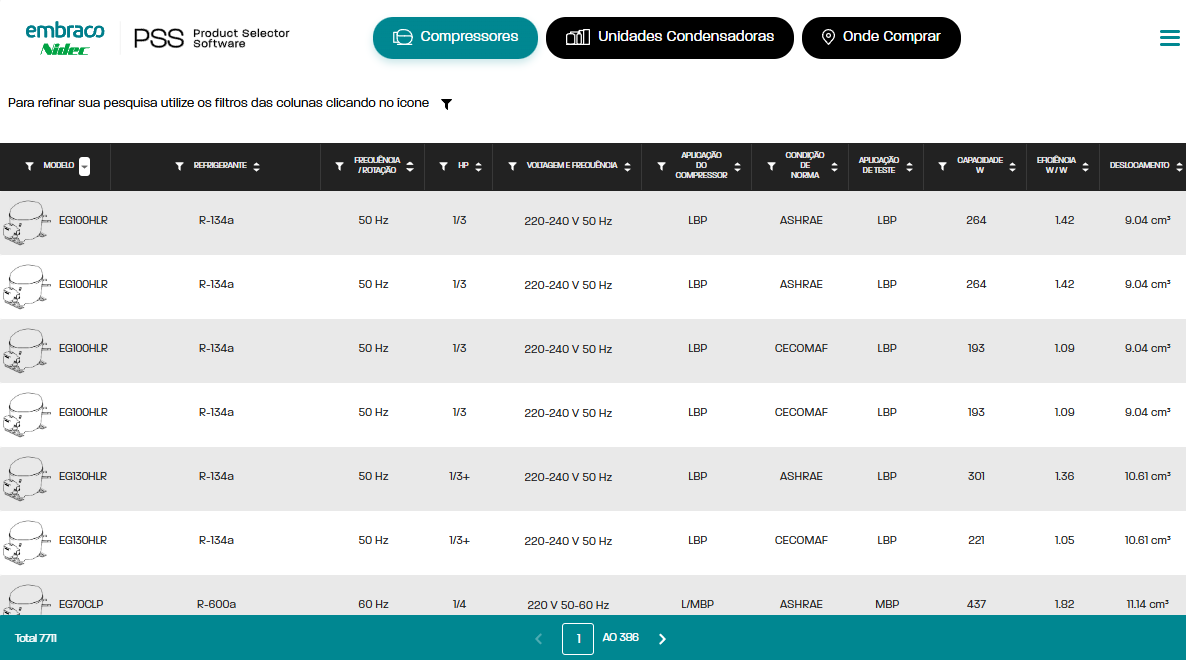
\includegraphics[width=0.8\linewidth]{Imagens/Desenvolvimento/PSS-embraco.png}
    \caption{Interface do seletor de produtos Embraco utilizado para pré-seleção dos compressores.}
    \label{fig:seletor de produtos}
\end{figure}

Os catálogos técnicos dos compressores pré-selecionados fornecem dados de desempenho obtidos em condições padronizadas de teste, incluindo temperaturas de evaporação e condensação, capacidade de refrigeração, consumo de potência elétrica e corrente nominal. Estes dados permitem uma análise comparativa detalhada do desempenho termodinâmico e econômico de cada modelo.

Foram selecionados quatro modelos de compressores herméticos que atendem aos requisitos de capacidade de refrigeração, apresentados na Tabela~\ref{tab:compressores escolhidos}.

\begin{table}[ht]
\centering
\begin{tabular}{|l|c|c|}
\hline
\textbf{Modelo} & \textbf{Potência Nominal [W]} & \textbf{Custo Estimado [R\$]} \\ \hline
EGAS80HLR & 240 & 650 \\ \hline
EGZS60HLP & 180 & 1340 \\ \hline
EGZS70HLC & 202 & 1130 \\ \hline
FFU70HAK & 221 & 600 \\ \hline
\end{tabular}
\caption{Compressores pré-selecionados para análise comparativa.}
\label{tab:compressores escolhidos}
\end{table}

\newpage

\section{Ciclo de Refrigeração Ideal}

Como referencial teórico para análise de desempenho, foi inicialmente considerado um ciclo de refrigeração ideal baseado no ciclo de Carnot reverso. Este ciclo representa o limite termodinâmico superior de eficiência para qualquer sistema de refrigeração operando entre duas fontes térmicas a temperaturas especificadas. O ciclo ideal de Carnot para refrigeração é composto por quatro processos reversíveis: compressão isentrópica do vapor saturado, condensação isotérmica à temperatura da fonte quente, expansão isentrópica do líquido saturado e evaporação isotérmica à temperatura da fonte fria, conforme ilustrado na Figura~\ref{fig: ciclo ideal}.

\begin{figure}[ht]
    \centering
    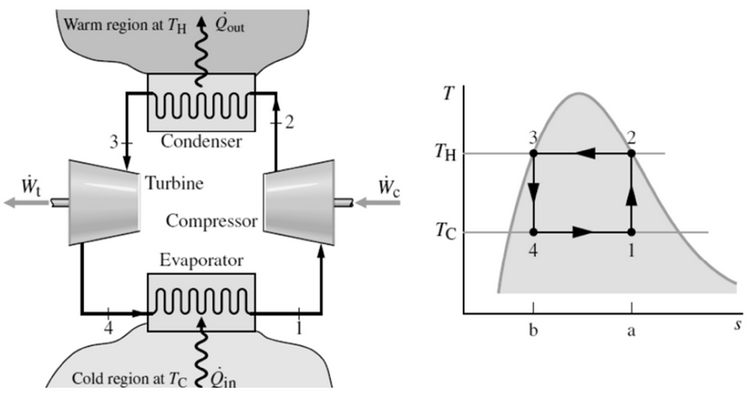
\includegraphics[width=0.6\linewidth]{Imagens/Desenvolvimento/carnot.png}
    \caption{Diagrama temperatura-entropia do ciclo ideal de Carnot para refrigeração.}
    \label{fig: ciclo ideal}
\end{figure}

Para o cálculo do coeficiente de performance (COP) de Carnot, consideraram-se as temperaturas de armazenamento do produto ($T_L = -25$°C = 248 K) e ambiente externo ($T_H = 35$°C = 308 K) como as temperaturas das fontes fria e quente, respectivamente. Esta simplificação representa o cenário termodinâmico mais favorável possível, desconsiderando irreversibilidades inerentes aos processos reais, como perdas por atrito, transferência de calor com diferença finita de temperatura e quedas de pressão.

O COP de Carnot é definido pela relação entre o efeito refrigerante ($\dot{Q}_L$) e o trabalho de compressão ($\dot{W}_c$), podendo ser expresso exclusivamente em função das temperaturas absolutas das fontes térmicas:

\begin{equation}
    \text{COP}_{\text{Carnot}} = \frac{T_L}{T_H - T_L} = \frac{\dot{Q}_L}{\dot{W}_c}
    \label{eq:cop carnot}
\end{equation}

Substituindo os valores de temperatura na Equação~\ref{eq:cop carnot}, obtém-se:

\begin{equation}
    \text{COP}_{\text{Carnot}} = \frac{248}{308 - 248} = 4,13
\end{equation}

A partir do COP de Carnot e da carga térmica determinada anteriormente (Equação~\ref{carga}), pode-se estimar a potência mínima teórica de compressão necessária:

\begin{equation}
    \dot{W}_{c,\text{ideal}} = \frac{\dot{Q}_L}{\text{COP}_{\text{Carnot}}} = \frac{202,6}{4,13} = 49,1~\text{W}
    \label{eq:potencia ideal}
\end{equation}

Este valor representa um limite termodinâmico inferior para a potência de compressão. Na prática, devido às irreversibilidades do ciclo real, à necessidade de diferenças de temperatura finitas nos trocadores de calor e às perdas mecânicas e elétricas do compressor, a potência real requerida será significativamente superior, tipicamente de 2 a 4 vezes maior que o valor ideal calculado.

\section{Ciclo de Refrigeração Real}

A partir dos parâmetros estabelecidos na análise preliminar, desenvolveu-se uma rotina computacional em Python para simular o ciclo de refrigeração por compressão de vapor considerando as não idealidades do processo real. O ciclo implementado segue a configuração apresentada na Figura~\ref{fig:ciclo padrão}, onde o fluido refrigerante R-134a entra no compressor como vapor saturado (estado 2), é comprimido isentropicamente até vapor superaquecido (estado 3), condensa isobaricamente até líquido saturado (estado 4) e sofre expansão isentálpica através de um dispositivo de expansão até a pressão de evaporação (estado 1).

\begin{figure}[ht]
    \centering
    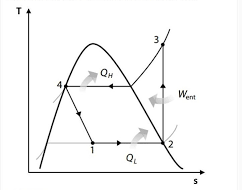
\includegraphics[width=0.6\linewidth]{Imagens/Desenvolvimento/Diagrama.png}
    \caption{Diagrama pressão-entalpia do ciclo real de refrigeração por compressão de vapor.}
    \label{fig:ciclo padrão}
\end{figure}


\subsection{Validação do Modelo com Dados de Catálogo}

Inicialmente, o programa foi validado utilizando as condições de teste padronizadas fornecidas nos catálogos técnicos dos compressores selecionados. Os fabricantes tipicamente apresentam dados de desempenho para combinações específicas de temperaturas de evaporação e condensação, permitindo a verificação da consistência do modelo desenvolvido. Esta etapa foi fundamental para assegurar a confiabilidade dos resultados e identificar quais compressores apresentam capacidade adequada para atender aos requisitos do projeto.

\subsection{Modelagem Termodinâmica do Ciclo}

A modelagem do ciclo real baseia-se na metodologia apresentada por \cite{paper_referencia}, que permite estimar a vazão mássica do refrigerante e a capacidade frigorífica efetiva do compressor a partir de suas características operacionais. A potência de compressão real é calculada pelo balanço de energia no compressor, considerando a variação de entalpia entre a sucção e descarga:

\begin{equation}
    \dot{W}_c = \dot{m}(h_3 - h_4)
    \label{W compressor}
\end{equation}

\noindent onde $\dot{m}$ é a vazão mássica de refrigerante, $h_3$ é a entalpia específica do vapor saturado na entrada do compressor e $h_4$ é a entalpia específica do vapor superaquecido na saída do compressor, calculada assumindo compressão isentrópica ($s_3 = s_4$) e conhecendo-se a pressão de condensação.

A capacidade de refrigeração do sistema é determinada pelo calor absorvido no evaporador:

\begin{equation}
    \dot{Q}_L = \dot{m}(h_2 - h_1)
    \label{capacidade evaporador}
\end{equation}

O coeficiente de performance do ciclo real é então calculado pela razão entre o efeito refrigerante e o trabalho de compressão:

\begin{equation}
    \text{COP}_{\text{real}} = \frac{\dot{Q}_L}{\dot{W}_c} = \frac{h_1 - h_4}{h_2 - h_1}
    \label{cop real}
\end{equation}

As propriedades termodinâmicas do R-134a em cada estado do ciclo (pressão, temperatura, entalpia e entropia) foram calculadas utilizando a biblioteca CoolProp, que implementa equações de estado de alta precisão. As Figuras \ref{fig:ciclo comp 1} e \ref{fig:ciclo comp 2} demonstram os resultados obtidos.

Para efeito de comparação e quantificação das perdas associadas às irreversibilidades do ciclo real, calculou-se paralelamente o COP do ciclo ideal de Carnot operando entre as mesmas temperaturas das fontes térmicas. A eficiência termodinâmica ou eficiência de segunda lei ($\eta_{II}$) do ciclo real pode então ser expressa como:

\begin{equation}
    \eta_{II} = \frac{\text{COP}_{\text{real}}}{\text{COP}_{\text{Carnot}}}
    \label{eficiencia segunda lei}
\end{equation}


Esta análise permite identificar o potencial de melhoria do sistema e quantificar o impacto das irreversibilidades no desempenho global do ciclo de refrigeração.

\begin{figure}[ht]
    \centering
    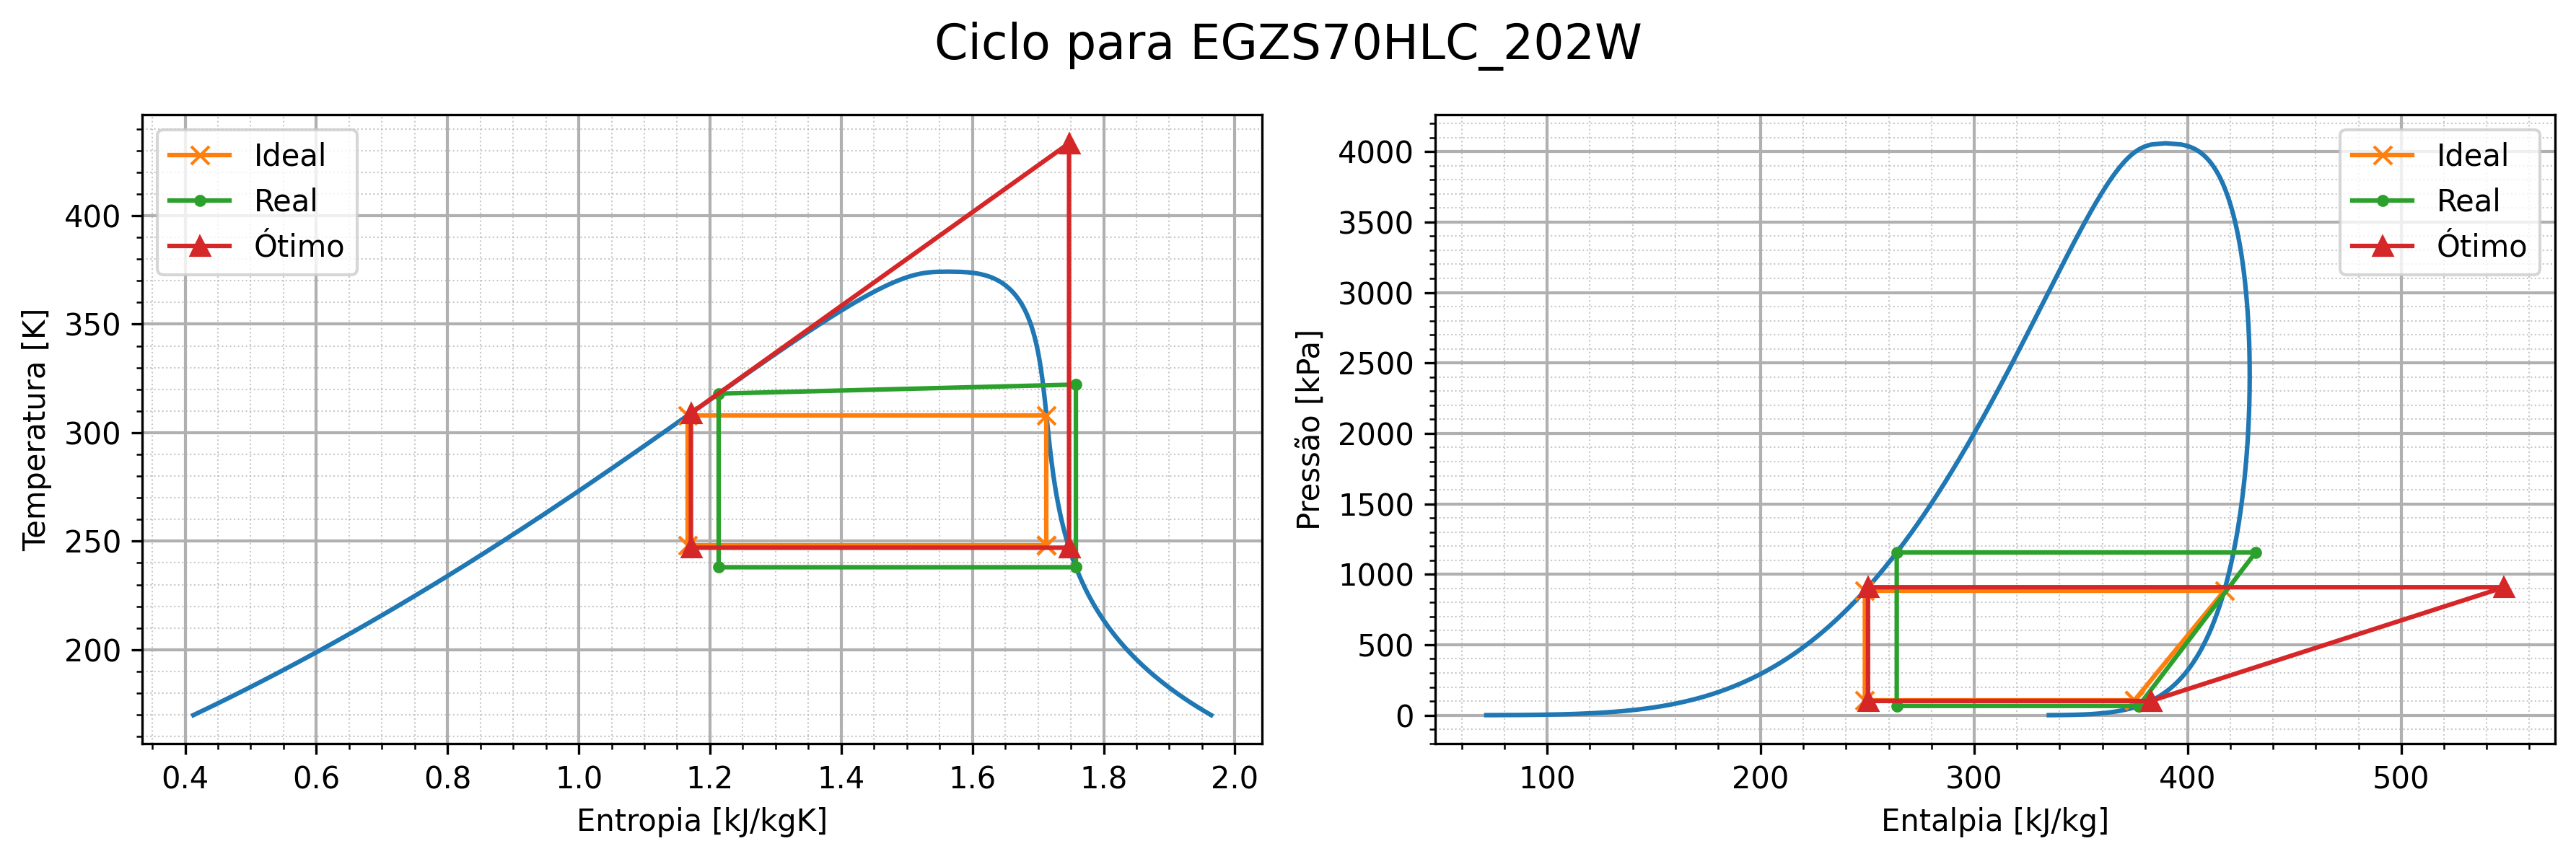
\includegraphics[width=\linewidth]{Imagens/Desenvolvimento/ciclo_EGZS70HLC_202W.png}
    \caption{Ciclo para o EGZS70HLC.}
    \label{fig:ciclo comp 1}
\end{figure}
Apenas os compressores \ref{fig:ciclo comp 1} e \ref{fig:ciclo comp 2} convergiram a resultados aceitáveis, gerando dúvidas no método utilizado.


\begin{figure}[ht]
    \centering
    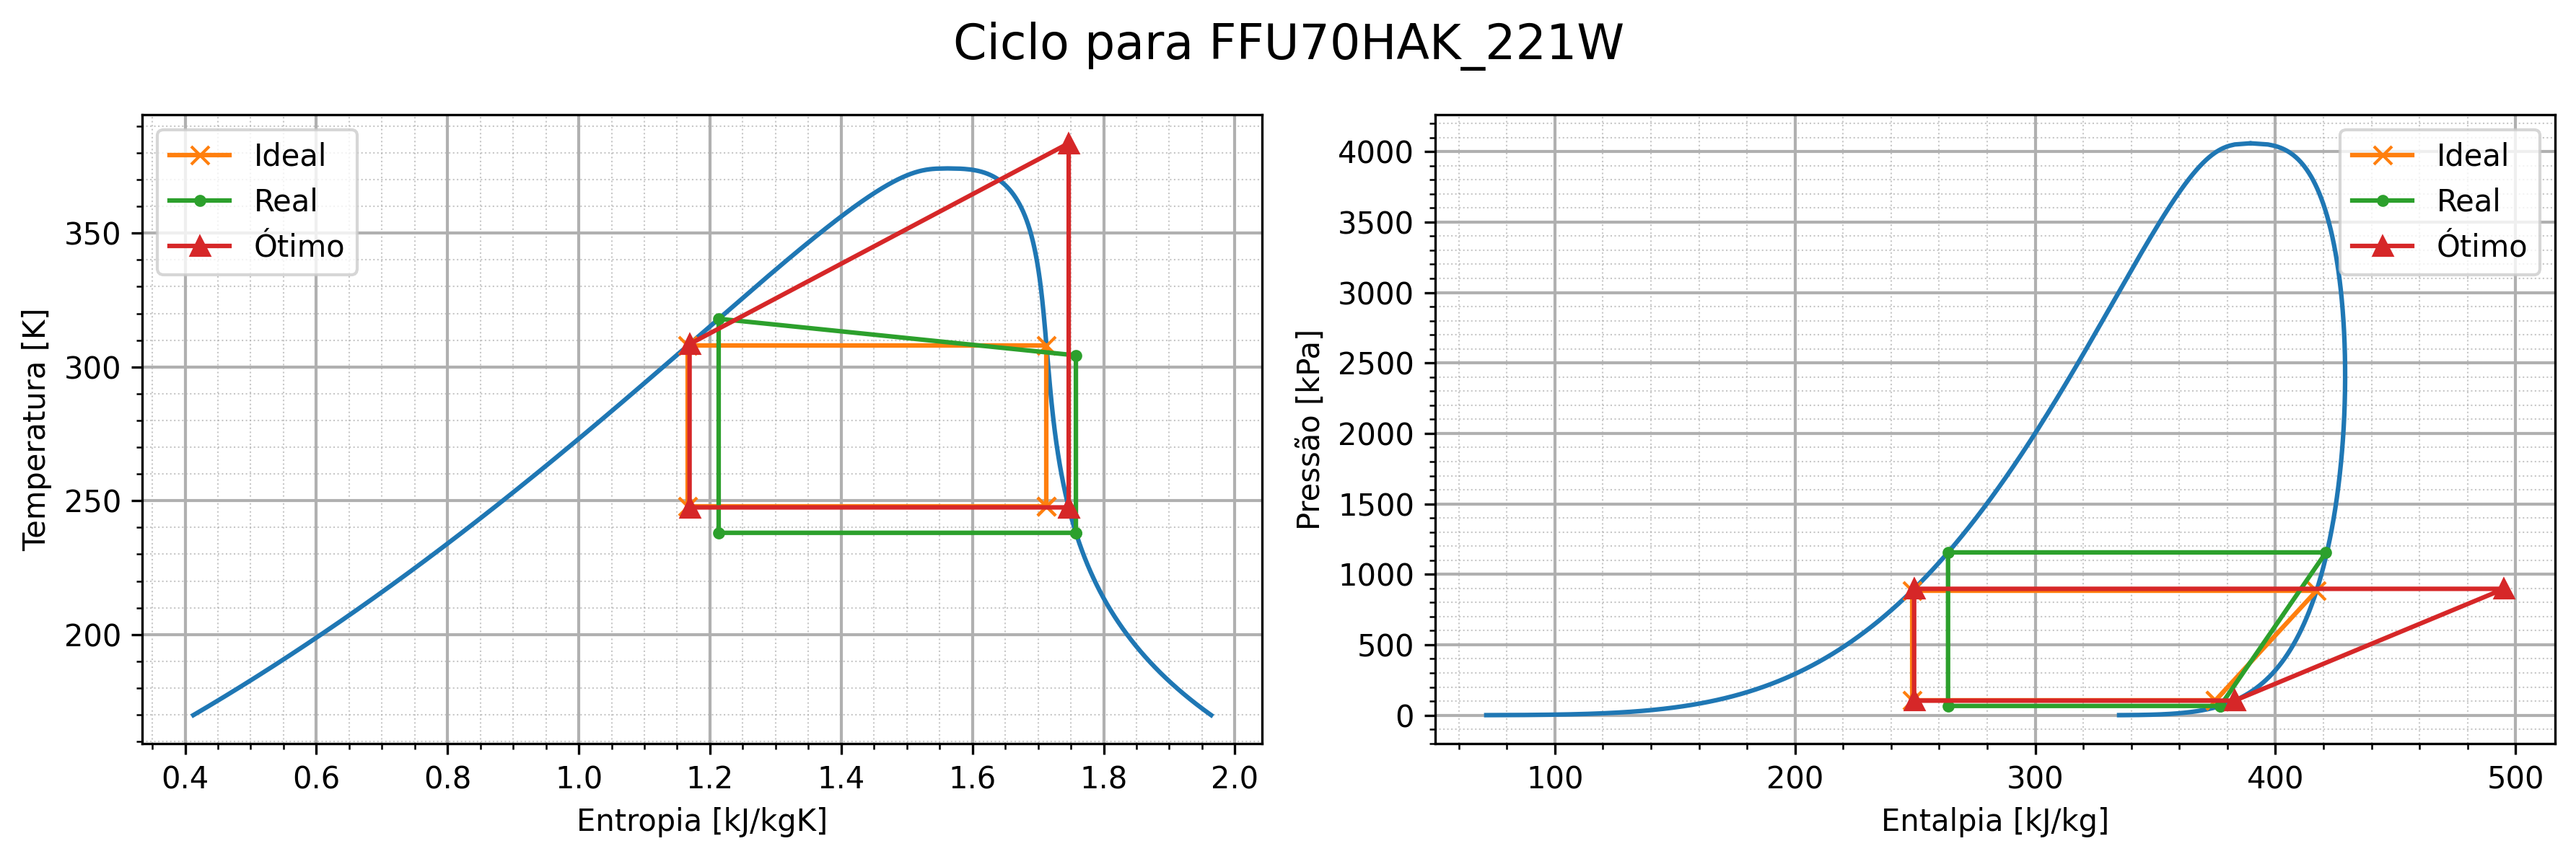
\includegraphics[width=\linewidth]{Imagens/Desenvolvimento/ciclo_FFU70HAK_221W.png}
    \caption{Ciclo para o FFU70HAK.}
    \label{fig:ciclo comp 2}
\end{figure}



Foi desenvolvida uma rotina de otimização utilizando a ferramenta \textit{Minimize} do pacote \textit{Scipy}, que foi utilizado para variar as temperaturas do condensador e do compressor a fim de minimizar o gasto energético, identificando a maior eficiência. Infelizmente os resultados não foram como esperado, resultando em temperatura muito similares com o ciclo de Carnot, porém com eficiência muito baixas, os resultados obtidos estão com a legenda "ótimo".


A análise comparativa entre os diferentes ciclos revela diferenças significativas nos parâmetros de desempenho. A rotina computacional desenvolvida calcula sistematicamente a vazão mássica de refrigerante ($\dot{m}$), potência de compressão ($\dot{W}_c$), coeficiente de performance (COP) e capacidade frigorífica ($\dot{Q}_L$) para os ciclos real e otimizado com dados de catálogo e otimizado, conforme apresentado nas Figuras~\ref{fig:barras fluxo massa} a~\ref{fig:barras Ql}.

\begin{figure}[ht]
    \centering
    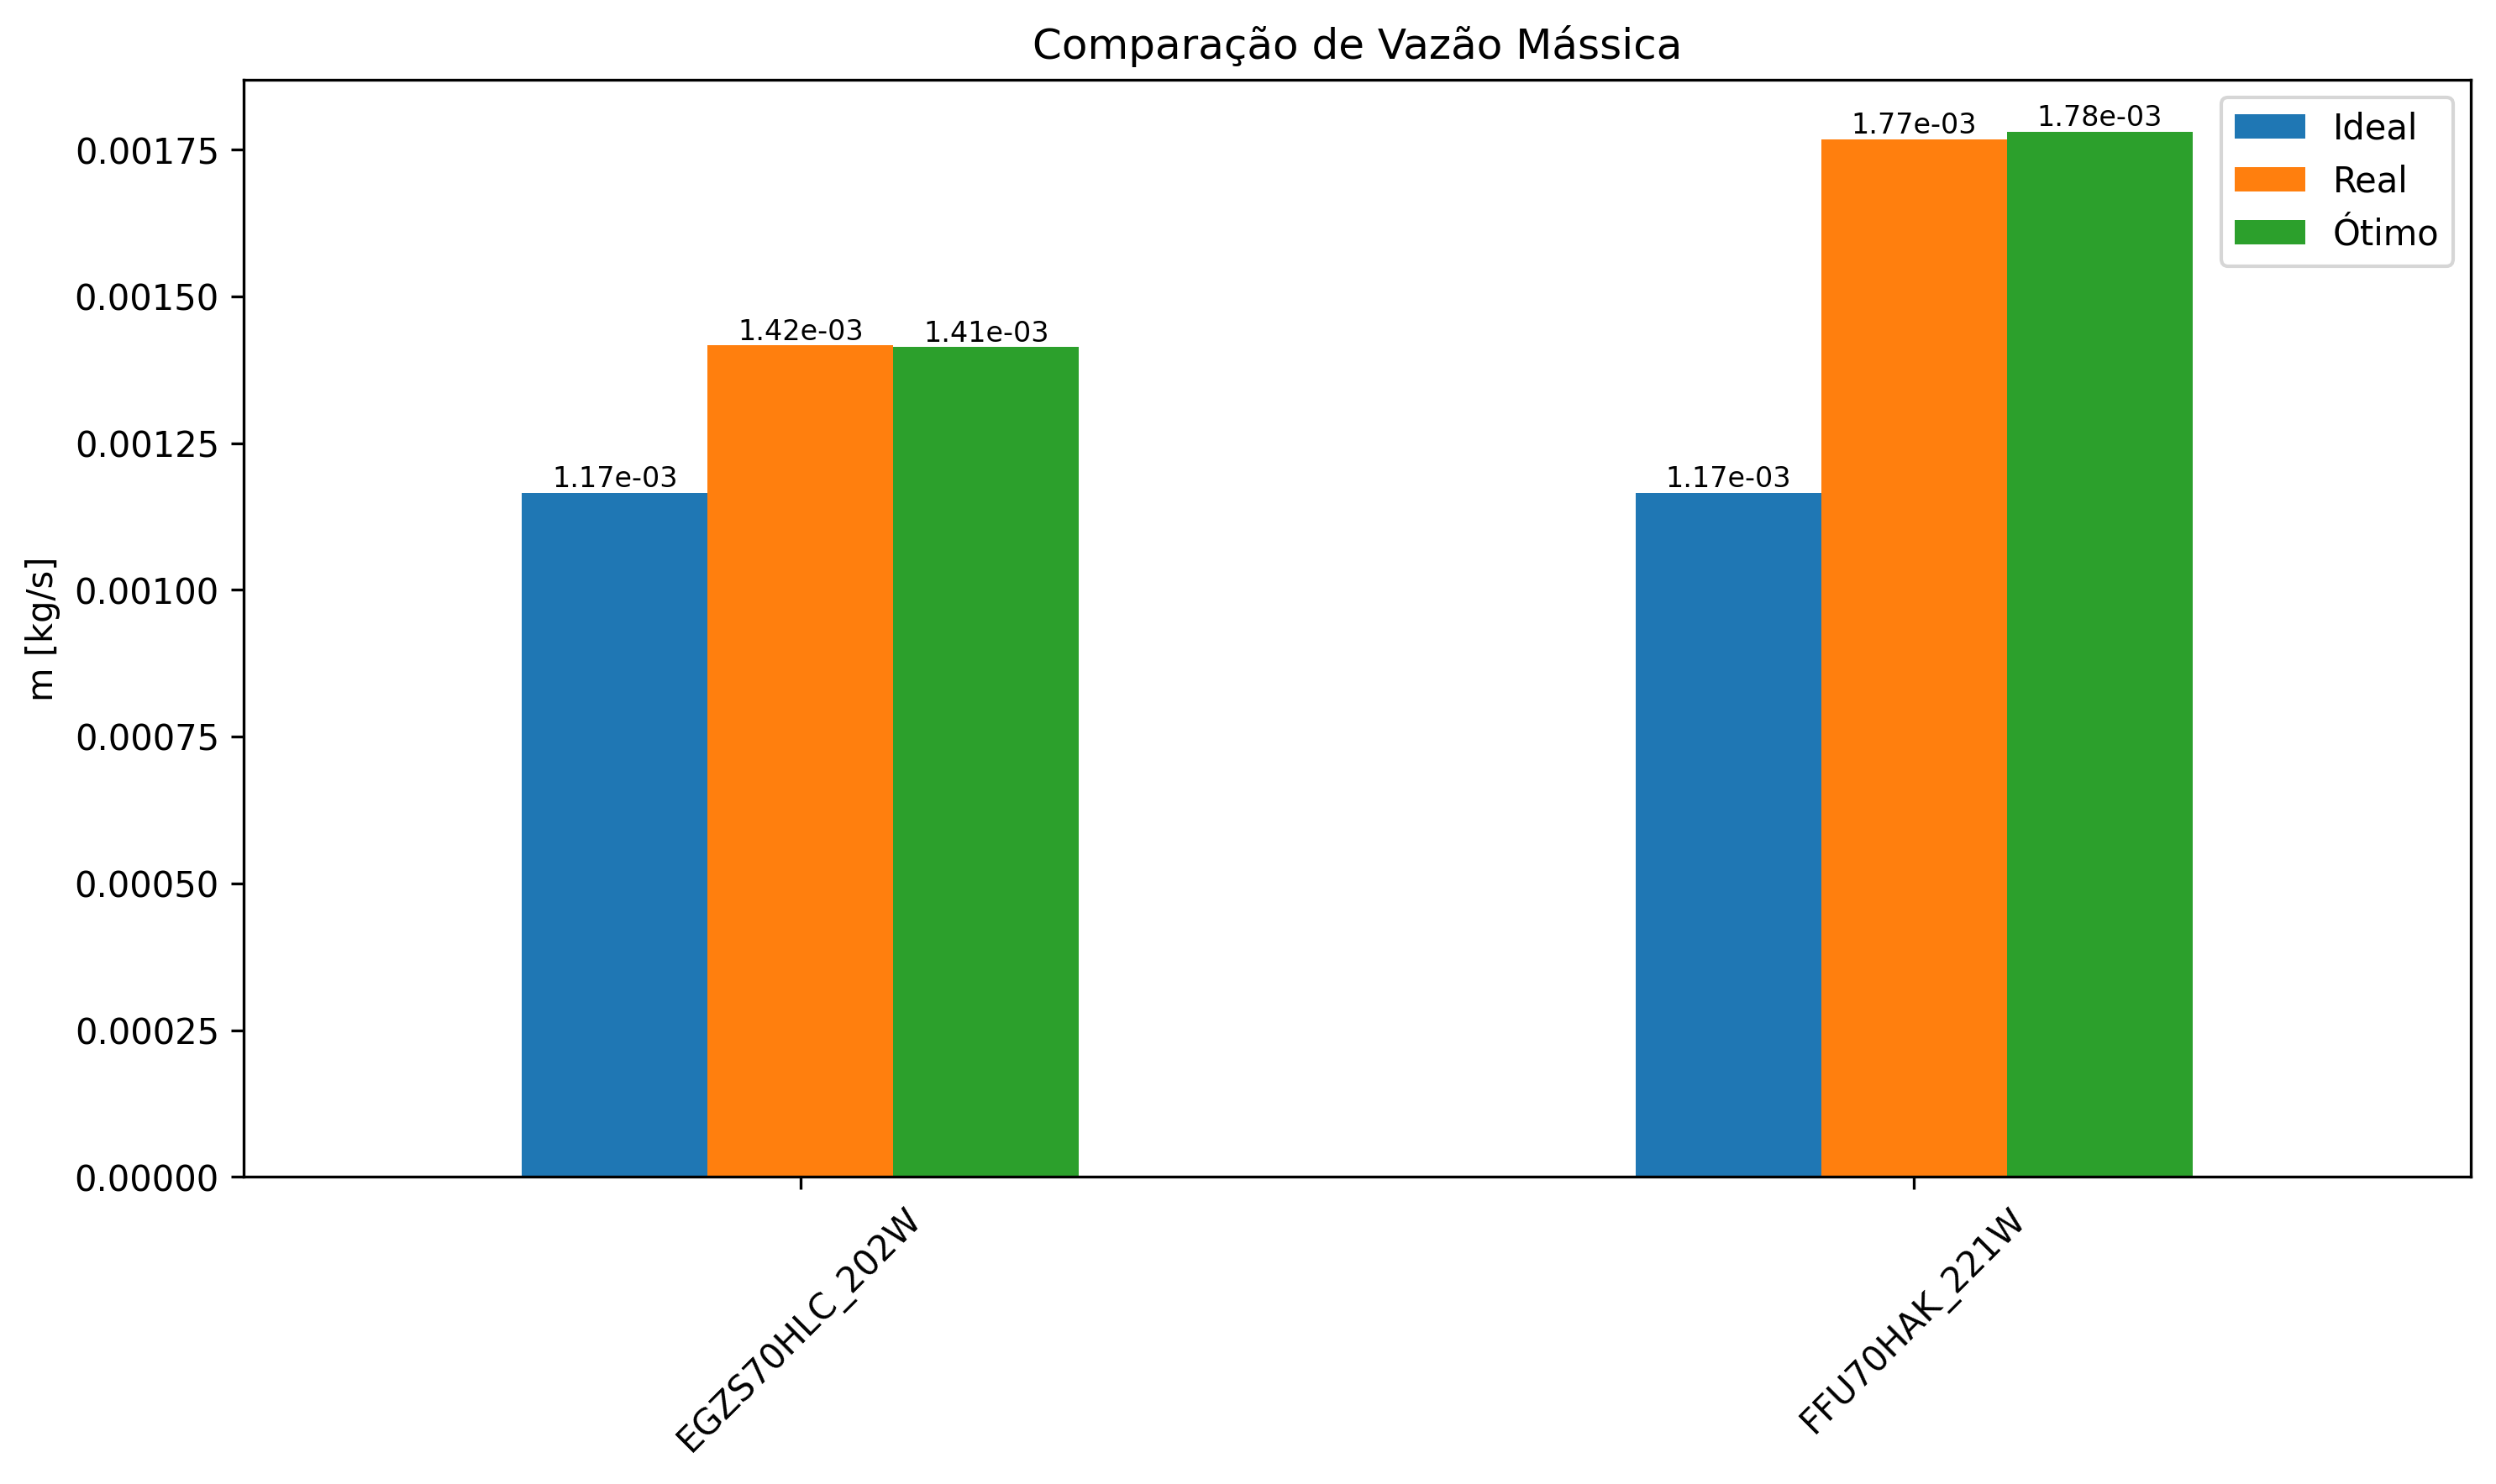
\includegraphics[width=0.8\linewidth]{Imagens/Desenvolvimento/barras_m.png}
    \caption{Comparação da vazão mássica de refrigerante entre os ciclos ideal, real e otimizado para os compressores selecionados.}
    \label{fig:barras fluxo massa}
\end{figure}

\begin{figure}[ht]
    \centering
    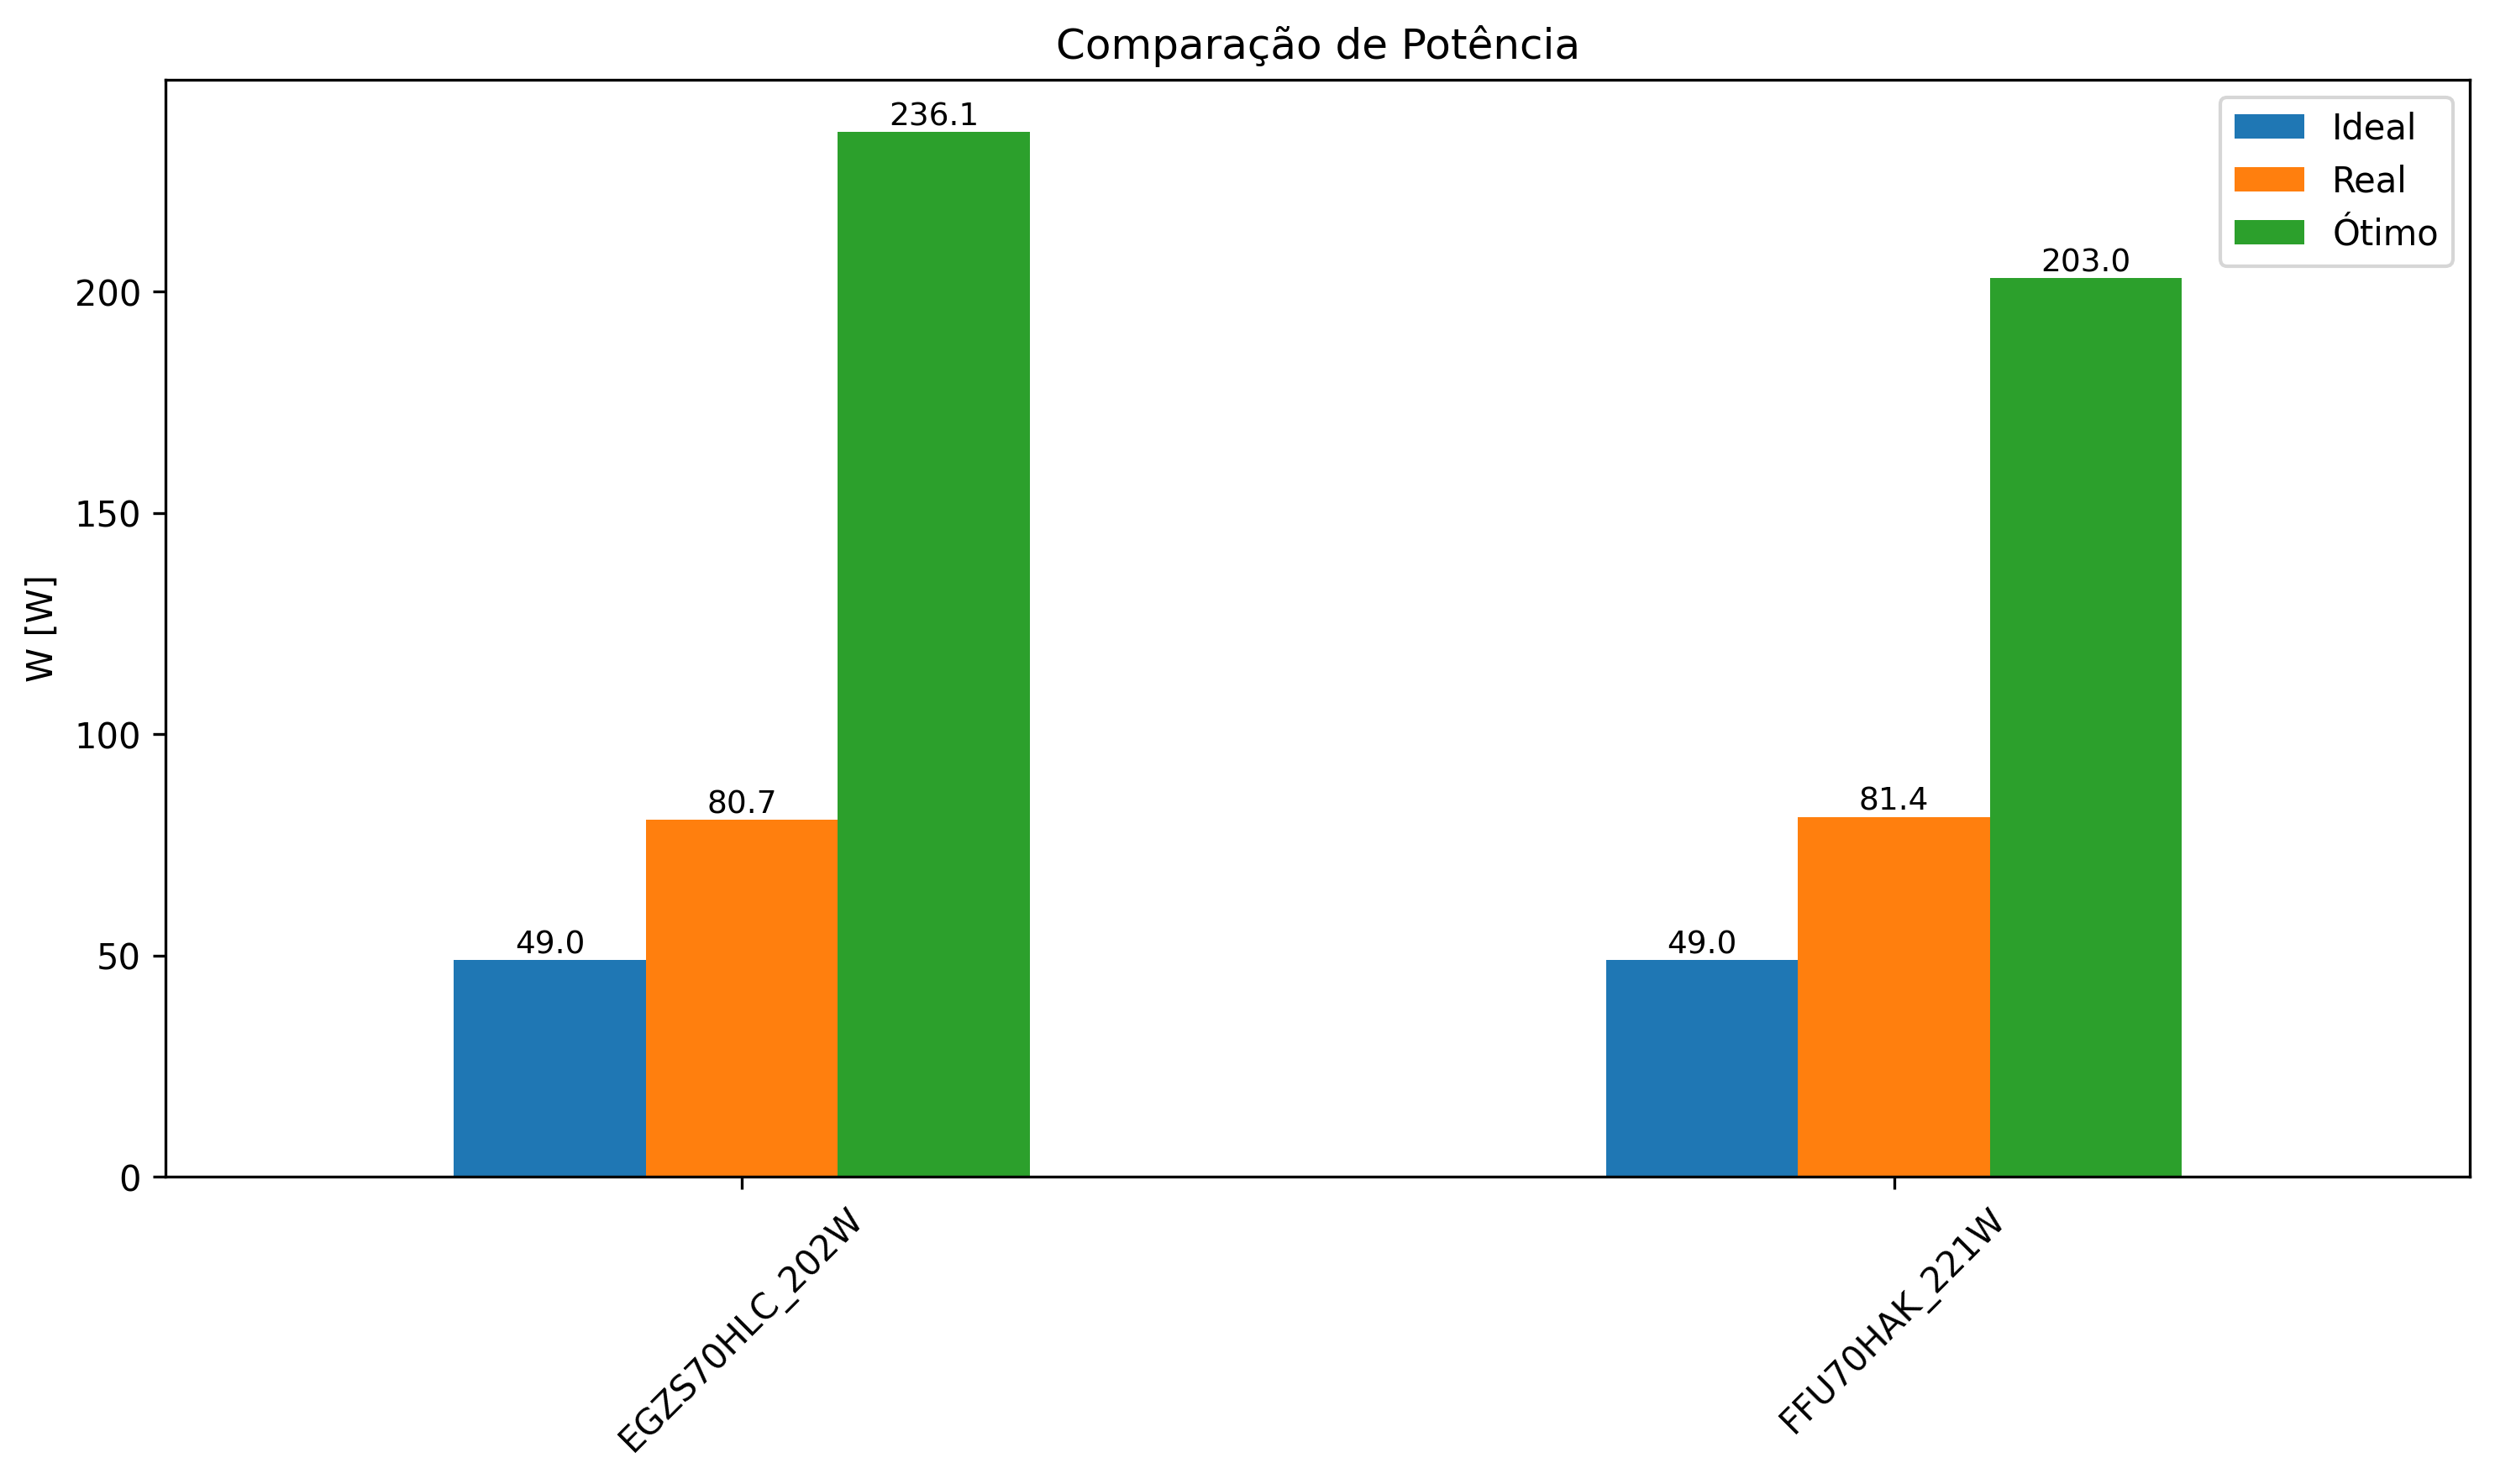
\includegraphics[width=0.8\linewidth]{Imagens/Desenvolvimento/barras_W.png}
    \caption{Comparação da potência de compressão entre os ciclos analisados.}
    \label{fig:barras W}
\end{figure}

\begin{figure}[ht]
    \centering
    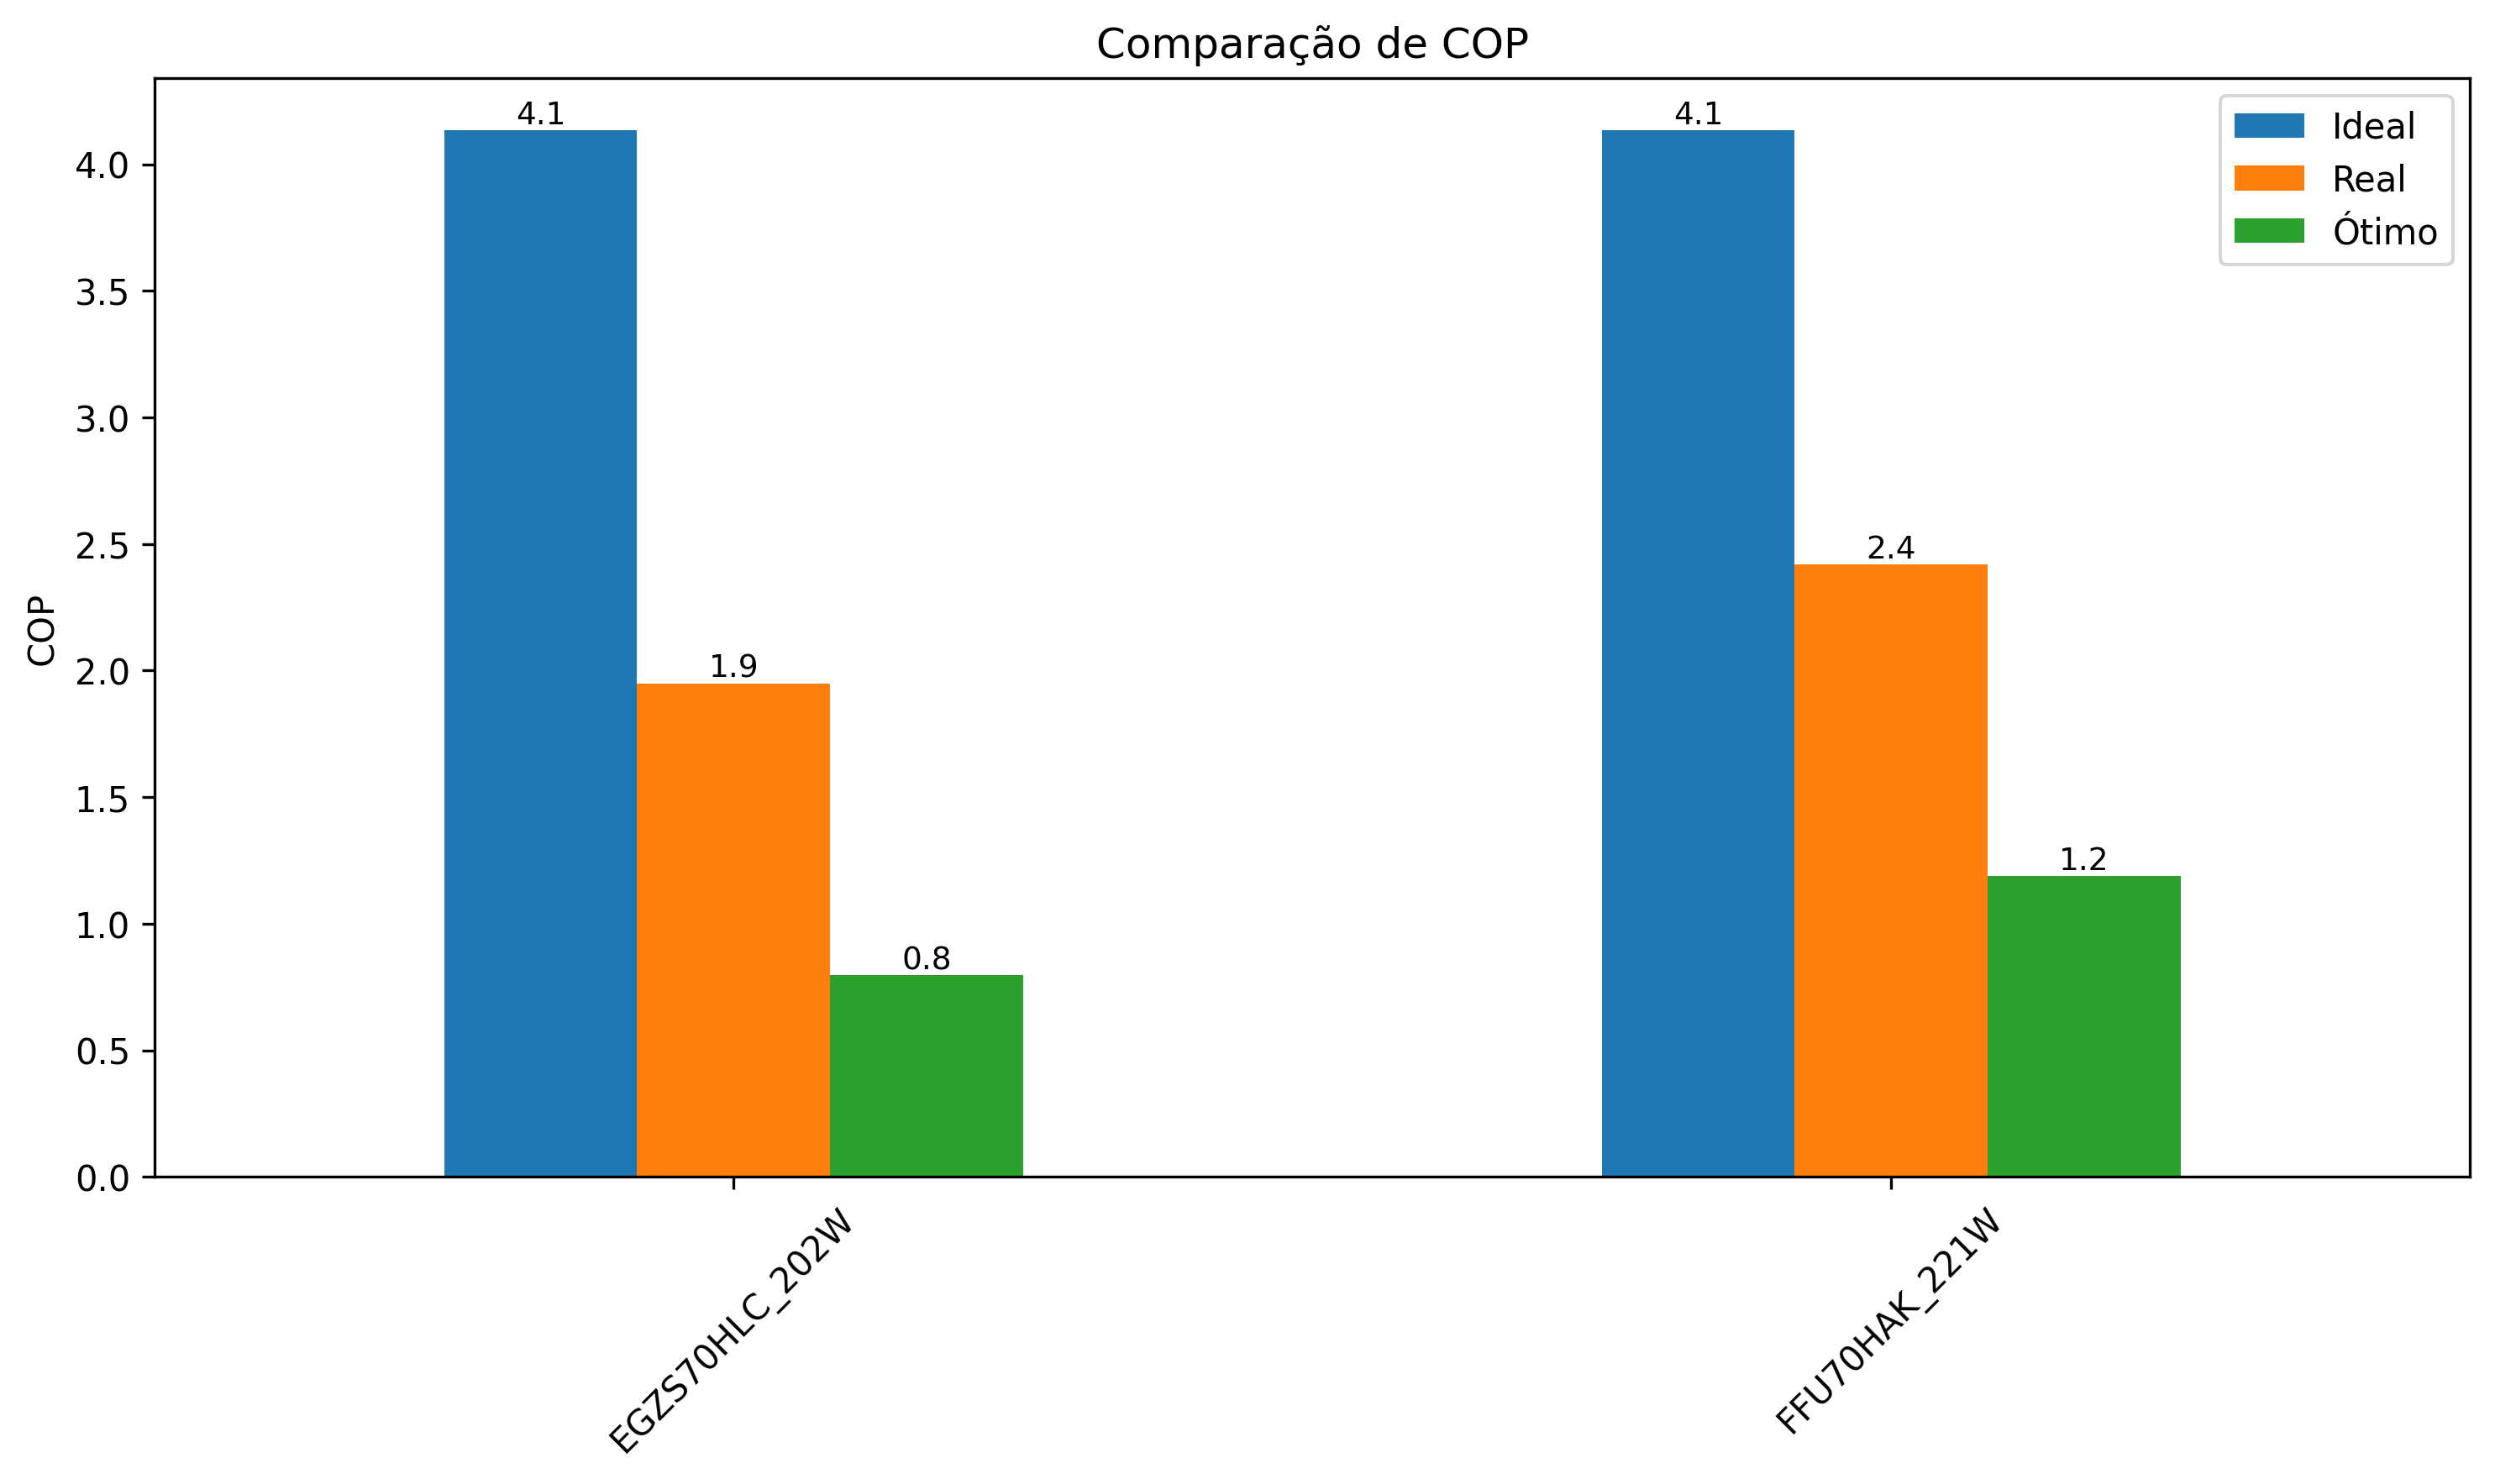
\includegraphics[width=0.8\linewidth]{Imagens/Desenvolvimento/barras_COP.png}
    \caption{Comparação do coeficiente de performance (COP) entre os diferentes ciclos.}
    \label{fig:barras COP}
\end{figure}

\begin{figure}[ht]
    \centering
    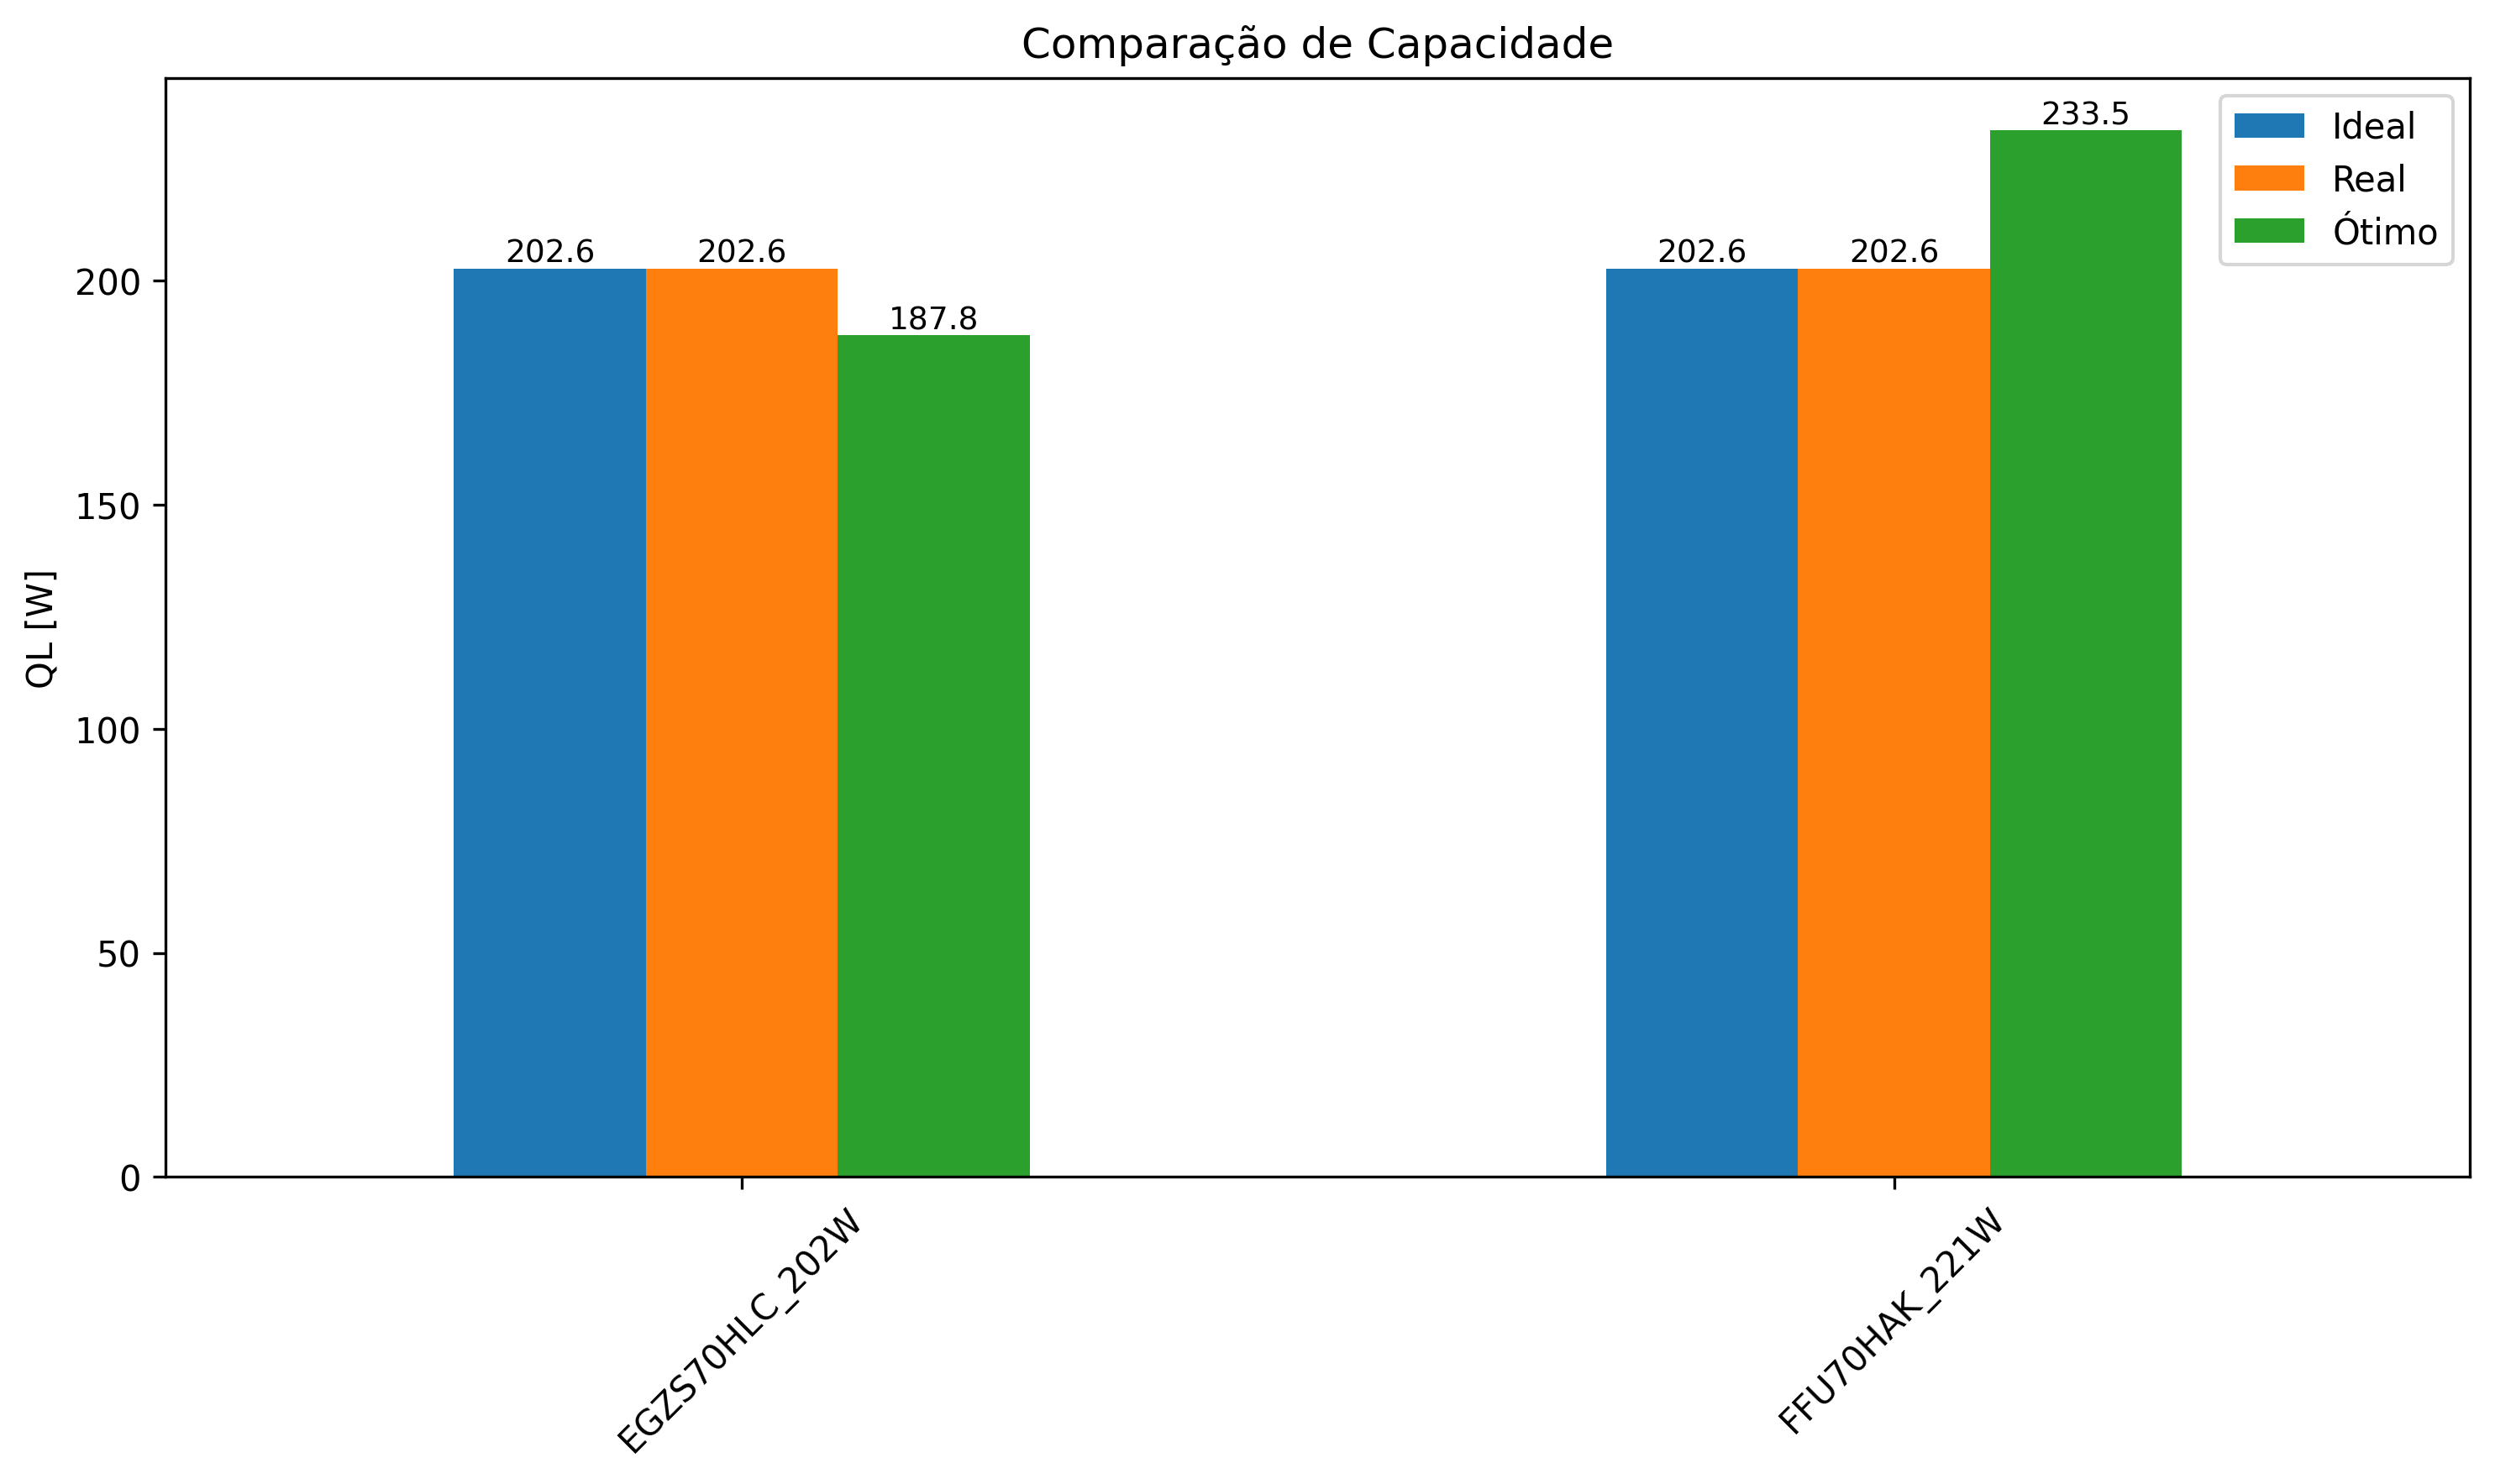
\includegraphics[width=0.8\linewidth]{Imagens/Desenvolvimento/barras_QL.png}
    \caption{Comparação da capacidade frigorífica entre os ciclos estudados.}
    \label{fig:barras Ql}
\end{figure}

\subsection{Análise dos Resultados}

Os resultados apresentados nas Figuras~\ref{fig:barras fluxo massa} a~\ref{fig:barras Ql} demonstram comportamento coerente com a teoria termodinâmica de ciclos de refrigeração, permitindo identificar o impacto das irreversibilidades nos parâmetros de desempenho:

\textbf{Vazão mássica ($\dot{m}$):} O ciclo ideal de Carnot apresenta a menor vazão mássica necessária, uma vez que opera com a máxima eficiência termodinâmica possível. Os ciclos real e otimizado requerem vazões superiores para fornecer a mesma capacidade frigorífica, compensando as perdas por irreversibilidades, como expansão isentálpica, superaquecimento do vapor na descarga do compressor e diferenças finitas de temperatura nos trocadores de calor.

\textbf{Coeficiente de Performance (COP):} O ciclo de Carnot estabelece o limite superior teórico de eficiência, servindo como referencial para avaliar o desempenho dos ciclos reais. A diferença entre o COP de Carnot e o COP real quantifica o efeito combinado de todas as irreversibilidades presentes no sistema.

\textbf{Potência de compressão ($\dot{W}_c$):} O ciclo ideal requer a menor potência de compressão devido à sua máxima eficiência. O ciclo real demanda potência significativamente superior devido às perdas já mencionadas, enquanto o ciclo otimizado busca um compromisso entre capacidade frigorífica e consumo energético através da seleção apropriada das condições operacionais.

\textbf{Capacidade frigorífica ($\dot{Q}_L$):} Observa-se que os diferentes ciclos fornecem capacidades frigoríficas distintas devido às variações na eficiência volumétrica do compressor e no efeito refrigerante específico, influenciados pelas condições de evaporação e condensação adotadas.

A Tabela~\ref{tab:eficiencias termo} apresenta as eficiências termodinâmicas calculadas para dois dos compressores analisados, tanto nas condições reais de catálogo quanto nas condições otimizadas. A eficiência $\eta_{II}$ representa a razão entre o COP real e otimizado em relação ao COP de Carnot, indicando o quão próximo o sistema opera do limite termodinâmico ideal.

\begin{table}[ht]
\centering
\begin{tabular}{|l|c|c|}
\hline
\textbf{Modelo} & \textbf{$\eta_{II}$ Real [\%]} & \textbf{$\eta_{II}$ Otimizado [\%]} \\ \hline
EGZS70HLC & 46,3 & 29,2 \\ \hline
FFU70HAK & 58,5 & 19,5 \\ \hline
\end{tabular}
\caption{Eficiências termodinâmicasdos compressores nas condições real e otimizada.}
\label{tab:eficiencias termo}
\end{table}

Observa-se que as eficiências termodinâmicas situam-se na faixa de 19,5\% a 58,5\%, valores típicos para sistemas de refrigeração operando com elevadas razões de compressão. A redução da eficiência no ciclo otimizado em relação ao ciclo real deve-se a interpolação do banco de dados do fabricante, talvez representando melhor um ciclo real.













% -----------------------------------------------------------------
% ELEMENTOS PÓS-TEXTUAIS
% -----------------------------------------------------------------
\postextual

% Você pode comentar os elementos que não deseja em seu trabalho;

% Referências bibliográficas

%Notar que os autores continuam sendo transpostos em maiúsculas, como preconiza a ABNT NBR 6023:2002. 
%Se, no entanto, não desejar seguir esta regra,
%crie um novo arquivo .bst (por exemplo, novoestilo.bst)a partir do estilo
%usado (abntex2-cite-alf ou abntex2-cite-num) e retire todas as expressões
%"u" change.case$, lembrando-se de indicar o novo arquivo como estilo, por exemplo, 
%\bibliographystyle{novoestilo}, e colocar o arquivo criado na mesma
%pasta em que está compilando o documento.

% Arquivo alterado para citação (Autor, Ano) ao invés de (AUTOR, Ano) conforme ABNT NBR 10520:2023
\bibliographystyle{abntex2-alf_revNBR2023.bst}	

\bibliography{abntex2-ref_UDESC_2020}	% Elemento Obrigatório

% % ----------------------------------------------------------
% Glossário
% ----------------------------------------------------------

%Consulte o manual da classe abntex2 para orientações sobre o glossário.

%\glossary




% ----------------------------------------------------------
% Glossário (Formatado Manualmente)
% ----------------------------------------------------------

\chapter*{GLOSSÁRIO}
\addcontentsline{toc}{chapter}{GLOSSÁRIO}

{ \setlength{\parindent}{0pt} % ambiente sem indentação

\textbf{Ardósia}: Rocha metamórfica sílico-argilosa formada pela transformação da argila sob pressão e temperatura, endurecida em finas lamelas.

\textbf{Arenito}: rocha sedimentária de origem detrítica formada de grãos agregados por um cimento natural silicoso, calcário ou ferruginoso que comunica ao conjunto em geral qualidades de dureza e compactação.

\textbf{Feldspato}: grupo de silicatos de sódio, potássio, cálcio ou outros elementos que compreende dois subgrupos, os feldspatos alcalinos e os plagioclásios.






} % fim ambiente sem indentação


				% Elemento Opcional
% 
% ----------------------------------------------------------
% Apêndices
% ----------------------------------------------------------

% ---
% Inicia os apêndices
% ---
\begin{apendicesenv}

% Imprime uma página indicando o início dos apêndices
%\partapendices

% ----------------------------------------------------------
\chapter{TÍTULO}
% ----------------------------------------------------------


\end{apendicesenv}
% ---				% Elemento Opcional
% 
% ----------------------------------------------------------
% Anexos
% ----------------------------------------------------------
%
% ---
% Inicia os anexos
% ---
\begin{anexosenv}

% Imprime uma página indicando o início dos anexos
%\partanexos

% ---
\chapter{TÍTULO}
% ---



\end{anexosenv}
				% Elemento Opcional
% 
%%---------------------------------------------------------------------
%% INDICE REMISSIVO
%%---------------------------------------------------------------------

%\phantompart
%\printindex

%---------------------------------------------------------------------

%%---------------------------------------------------------------------
%% INDICE REMISSIVO (Formatado Manualmente)
%%---------------------------------------------------------------------

\chapter*{ÍNDICE}
\addcontentsline{toc}{chapter}{ÍNDICE}

{ \setlength{\parindent}{0pt}  % ambiente sem indentação
	
Andesito, 22, 50, 73

Argila, 52, 75, 121

Basalto, 25, 230, 235

	
	
	
	
} % fim ambiente sem indentação


		% Elemento Opcional



\end{document}

% -----------------------------------------------------------------
% Fim do Documento
% -----------------------------------------------------------------	